%%
%% This is file `example/bare_thesis.tex',
%% generated with the docstrip utility.
%%
%% The original source files were:
%%
%% install/buptgraduatethesis.dtx  (with options: `bare-thesis')
%% 
%% This file is a part of the example of BUPTGraduateThesis.
%% 

\documentclass[degree=master,classlevel=open,mathfont=mathptmx,dedication=false,chapbib=false,finish=print,driver=xetex]{buptgraduatethesis}

%% 自定义导言区
%% 在这里添加你需要的宏包、自定义命令、环境等
%% \usepackage{...}
%% \DeclareMathOperator{\CT}{H}
%% \DeclareMathOperator{\Cov}{Cov}
\usepackage{listings}
\usepackage{minted}
\usepackage{color}
\usepackage{graphicx}
\usepackage{pythonhighlight}

\usepackage{algorithm}
\usepackage{algorithmicx}
\usepackage{algpseudocode}
\usepackage{amsmath}

\definecolor{bg}{rgb}{0.95,0.95,0.95}
\floatname{algorithm}{伪代码}
\renewcommand{\algorithmicrequire}{\textbf{输入:}}
\renewcommand{\algorithmicensure}{\textbf{输出:}}

\def\BUPTThesis{\textsc{BUPT}\-\textsc{Thesis}}

%% 在这里添加图片文件搜索目录
\graphicspath{{../}}
%% 自定义导言区结束

%% 加载缩略语定义
%%
%% This is file `example/metadata.tex',
%% generated with the docstrip utility.
%%
%% The original source files were:
%%
%% install/buptgraduatethesis.dtx  (with options: `metadata')
%% 
%% This file is a part of the example of BUPTGraduateThesis.
%% 

%% 涉密论文保密年限
\classdur{三年}

%% 学号
\studentid{2014111409}

%% 论文题目
\ctitle{基于SDN的多租户虚拟网络定制化的研究与实现}
\etitle{Example of BUPT Graduate Thesis \LaTeXe{} Template}

%% 申请学位
\cdegree{工学硕士}

%% 院系名称
\cdepartment{网络技术研究院}

%% 专业名称
\cmajor{信息与通信工程}

%% 你的姓名
\cauthor{李凯}

%% 你导师的姓名
\csupervisor{廖建新}

%% 日期自动生成,也可以取消注释下面一行,自行指定日期
%\cdate{\CJKdigits{2015}年\CJKnumber{12}月\CJKnumber{26}日}
\cdate{2015年12月26日}

%% 中文摘要
\cabstract{%
  中、英文摘要位于声明的次页,摘要应简明表达学位论文的内容要点,体现研究工作的核心思想。
  重点说明本项科研的目的和意义、研究方法、研究成果、结论,注意突出具有创新性的成果和新见解的部分。

  关键词是为文献标引工作而从论文中选取出来的、用以表示全文主题内容信息的术语。
  关键词排列在摘要内容的左下方,具体关键词之间以均匀间隔分开排列,无需其它符号。
}

%% 中文关键词,关键词之间用 \kwsep 分割
\ckeywords{\TeX \kwsep \LaTeX \kwsep xeCJK \kwsep 模板 \kwsep 排版 \kwsep 论文}

%% 英文摘要
\eabstract{%
  The Chinese and English abstract should appear after the declaration page.
  The abstract should present the core of the research work, especially the purpose and importance of the research, the method adopted, the results, and the conclusion.

  Key words are terms selected for documentation indexing, which should present the main contributions of the thesis.
  Key words are aligned at the bottom left side of the abstract content.
  Key words should be seperated by spaces but not any other symbols.
}

%% 英文关键词,也用 \kwsep 分割
\ekeywords{%
  \TeX \kwsep \LaTeX \kwsep xeCJK \kwsep template \kwsep typesetting \kwsep thesis}


\loadglsentries{acronyms}

%% 攻读学位期间发表论文
%% 用 \newcite{<suffix>}{<caption>} 声明不同的论文类型(例如: 期刊论文、会议论文等)。每一个类型的对应的 .bib 文件用 \bibliography<suffix> 命令加载,用 \nocite<suffix> 命令引用。具体请参考 pubs.tex 中的示例
\newcite{jrnl}{期刊论文}
\newcite{conf}{会议论文}
\newcite{patent}{专利}

\begin{document}
%% 声明前置部分
\makefrontmatter

%% 生成主要符号对照表
%%%
%% This is file `example/notations.tex',
%% generated with the docstrip utility.
%%
%% The original source files were:
%%
%% install/buptgraduatethesis.dtx  (with options: `notations')
%% 
%% This file is a part of the example of BUPTGraduateThesis.
%% 

\begin{listofnotations}
\item [$(\cdot)^*$] 复共轭
\item [$(\cdot)^{\mathrm T}$] 矩阵转置
\item [$(\cdot)^{\mathrm H}$] 矩阵共轭转置
\item [$\mathbf{X}$] 矩阵或向量
\item [$\mathcal{A}$] 集合
\item [$\mathcal{A}\times\mathcal{B}$]
  集合 $\mathcal{A}$ 与集合 $\mathcal{B}$ 的 Cartesian 积,即 $\mathcal{A}\times\mathcal{B}=\{(a,b):a\in\mathcal{A},b\in\mathcal{B}\}$
\end{listofnotations}


%% 主体部分
\mainmatter
%% 用\include{}命令引用各章.tex文件
%%
%% This is file `example/ch_intro.tex',
%% generated with the docstrip utility.
%%
%% The original source files were:
%%
%% install/buptgraduatethesis.dtx  (with options: `ch-intro')
%% 
%% This file is a part of the example of BUPTGraduateThesis.
%% 

\chapter{绪论}
\section{研究背景及意义}
随着互联网的发展,云数据中心的规模不断扩大,业务流量不断变化,如何为租户提供可编程的云数据中心网络,如何对云数据中心的流量进行有效的控制,提高带宽的利用率,降低成本,成为目前急需解决的问题。

\gls*{SDN}作为一种新兴的可编程网络架构\cite{SDN-0},有动态配置、可编程及快速响应的特点。其核心思想是将网络控制平面与数据转发平面分离,实现控制平面对数据平面的全局集中化控制;同时对外提供开放的可编程接口,为网络提供可编程能力。控制权的迁移使得底层构架能够抽象出来,各种应用和网络服务因此能将网络当作一个逻辑或虚拟实体,不再依赖于底层网络设备\cite{SDN-1},使得网络配置的自动化程度得到极大提高。通过应用SDN,除了网络的设计和操作变得简化,网络设备也得到简化,这些设备无需理解或处理成千上万的协议,只需要接受SDN控制器的指令即可。利用集中控制,网络管理员可以实时改变网络的行为,并且在几小时或几天内就可以部署新的应用和网络服务。

网络虚拟化\cite{Virtual-1}是一种将底层网络中的硬件以及配套的软件资源进行整合,形成统一管理实体的技术,通过虚拟网络资源到物理网络资源的映射,使得多个逻辑虚拟网络共享底层物理网络基础设施,为用户提供差异化服务。网络虚拟化技术是当今网络革新的重要技术之一。从概念上,网络虚拟化与SDN是互相独立的,但随着近几年网络技术的发展与融合,二者之间的联系变得越来越紧密,SDN的技术相关专题常会提及网络虚拟化技术,网络虚拟化问题的研究也时常会运用到SDN的概念,可见基于SDN的网络虚拟化技术已经成为网络技术研究领域的一个专门课题\cite{Virtual-2}。

OpenStack\cite{OpenStack-1}是由Rackspace和美国国家航空航天局(NASA)合作研发的用于搭建\gls*{IaaS}平台的云计算管理软件。旨在为公共及私有云的建设与管理提供软件的开源项目,主要提供计算、存储、网络服务。OpenStack支持几乎所有类型的云环境,项目目标是提供实施简单、可大规模扩展、丰富、标准统一的云计算管理平台。OpenStack通过各种互补的服务提供了\gls*{IaaS}的解决方案,每个服务提供API以进行集成\cite{OpenStack-2}。

在现有OpenStack云平台中,租户网络的创建与隔离仅限于服务器内部,OpenStack无法进行物理服务器之间数据中心网络的管控,跨服务器的通信通过隧道技术实现,该模式无法满足用户多样性的需求,同时无法实现云数据中心带宽资源的有效利用,时常会出现有些链路阻塞严重,而有些链路则处于空闲状态。

本文以此作为出发点,提出了一种基于SDN的多租户虚拟网络定制化管理机制,运用虚拟化技术,为租户提供相互隔离的\gls*{vSDN},完成云数据中心物理资源有效利用的同时,SDN网络由租户自有的控制器实现集中管控,租户可以实时监测当前的流量状况并根据流量状况自定义转发路径,实现对网络的灵活管控,在不降低云平台性能的前提下,实现了OpenStack云平台中租户网络的定制化操作,既提高了安全性,又可以根据当下链路的剩余带宽,进行链路的定制化,提高带宽的利用率。对于租户本身而言,真正实现了租户对全局网络的可控性。对于运营商来说,对物理网络的集中控制可以大大减小网络配置的繁琐性,可以对网络故障实现快速的排查,提高可扩展性。

\section{主要研究内容及创新点}
\subsection{研究内容}
本课题为实现基于SDN的云平台多租户虚拟网络定制化方案,将SDN集成到云数据中心,通过虚拟化技术,为租户提供了可编程的vSDN网络,vSDN网络由租户自有的SDN控制器进行集中管控,租户可以根据当前的链路状况,进行定制化流表的下发,真正实现对网络的灵活定制化操作。主要包括以下三个方面的研究内容:

第一、实现虚拟网络的创建:通过虚拟化技术,实现跨物理服务器,数据中心网络的虚拟化,虚拟网络支持SDN模式,由租户自己的SDN控制器实现集中管控,本文选用\gls*{OVX}\cite{OVX-1}实现虚拟网络的创建。对于底层物理设备来说,OVX是一个控制器;对于租户控制器来说,OVX可以看作是OpenFlow交换机的集合,租户控制器看到的只是一张虚拟网络。OVX最大的优势是紧密结合了SDN,可以发挥SDN的控制与转发分离的强大优势,将创建的虚拟网络指定SDN控制器,从而可以运用SDN的优势,实现对租户虚拟网络的管控。该部分主要对OVX进行二次开发,为其封装创建虚拟网络的API接口,同时,完成与OpenStack的集成,实现OVX对OpenStack虚拟机的集中管控。

第二、完成虚拟网络的集中控制:针对租户创建的vSDN网络,由租户自己的SDN控制器进行集中管控,本文为用户提供了集成Ryu\cite{Ryu-1}控制器的定制化镜像。本文为该控制器开发了测量剩余带宽、已用带宽、链路时延以及下发定制化流表的应用。租户可以进行网络带宽、时延的查询,根据当前网络的链路状态,选取一条最优的数据传输链路,下发定制化流表,从而实现数据传输的可控性。提高带宽利用率的同时,数据传输速率得到了很大的改善。

第三、云平台前端可视化操作:本文为实现租户的便捷操作,在OpenStack云平台上开放了可视化界面操作。其一是用来显示物理数据中心网络,并在数据中心网络上进行租户虚拟网络的创建操作,以及数据中心网络链路时延的显示工作。其二用于实现租户虚拟网络的拓扑展示,虚拟网络带宽、时延的展示,以及定制化链路的选取和流表的下发操作。使用户切身感受到操作的便捷性、对网络的可控性。

\subsection{创新点}
针对现有云平台数据中心的不足,本文主要实现了SDN与云平台的结合,将SDN的集中控制、网络的虚拟化集成到云平台中,实现了租户网络隔离的同时,租户可以对网络实现自由控制。相应的创新点主要涉及以下几个方面:

\begin{enumerate}
\item 对于云平台运营商来说,物理网络的集中控制,可以有效的减小网络配置的繁琐性,为数据中心规模的伸缩性提供了便利,对网络的状况可以进行实时监控,同时大大加快了网络的故障修复速度,通过控制侧的日志输出,以及错误模拟,实现快速故障排除。
\item 将虚拟化技术集成到云数据中心,为租户提供相互隔离的vSDN网络,该网络由租户自己的控制器实现集中控制。集中控制的实现,可以让租户指定灵活的数据包转发路径,以及灵活的转发策略。对于自身网络的变化也可以实现即时的应对措施。从而对现有的网络资源进行最有效的利用,减少了网络资源的浪费。租户之间的隔离性,保证了租户数据传输的安全性。
\item SDN模式下带宽时延的测量,首先基于包对技术,完成了虚拟网络的链路带宽测量,实现了细粒度的剩余带宽测量,精确度远远高于以前的模式;基于数据包统计的方法,实现了粗粒度的已用带宽的测量;完成了SDN架构下的时延测量。租户可以根据带宽、时延实现定制化链路的选取,有效的利用剩余带宽,降低数据传输时延,加快数据中心网络的传输速度。
\end{enumerate}

综上所述,基于SDN的云平台多租户虚拟网络定制化方案,对提高云数据中心的带宽利用率,为租户提供可编程的云网络是非常必要的,有助于实现租户网络的定制化操作,同时为运营商进行云数据中心的维护和配置提供了便利。

\section{研究生期间主要工作}
在攻读硕士研究生期间,本文作者认真学习专业相关课程,积极参与实验室的科研工作。认真学习了网络智能研究中心要求的基本课程并取得了满意的成绩,先后参与了实验室多个科研项目。主要的研究方向为智慧云平台的开发工作,在老师和师兄师姐的指导下,对研究课题进行了深入的探索,通过阅读书籍和学术论文夯实理论基础,并进行系统设计、实现和功能测试。主要科研经历和学术成果如下:

参与了国家重点实验室自主课题仪器设备研制类——面向无线业务的网络智能承载验证环境,开发智慧云平台,为租户提供自主可控的SDN云网络;在国家重点基础研究发展计划(973 计划)课题——智慧服务机理与理论中,负责新一代网络架构的调研和撰写工作。

以第一作者的身份发表了两篇EI检索论文,具体为:通过对多租户虚拟网络定制化机制的研究,发表了学术论文《MVNC: A SDN-based Multi-tenant Virtual Network Customization Mechanism in Cloud Data Center》,在论文中提出了一种MVNC的多租户虚拟网络定制化机制,论文已发表于IEEE。通过对\gls*{PSO}及网路虚拟化的研究,撰写了学术论文《A PSO-Based Virtual Network Customization for Multi-tenant Cloud Services》,在论文中,提出了一种基于PSO算法的网络虚拟化方案,实验证明相对于传统的基于最短路径的虚拟化算法,性能得到很大提升。同时,在此基础上,完成了多租户云服务中虚拟网络的定制化。论文已被录用。
\section{论文组织结构}
论文总共包括五章,具体内容组织如下:

第一章主要概述了研究背景、意义以及研究的主要内容,包括SDN、OpenStack的背景介绍,本文的主要研究内容以及基于SDN云平台多租户虚拟网络定制化的意义、创新点。

第二章主要介绍了SDN、网络虚拟化及OpenStack的相关技术。首先介绍了OpenFlow 协议,OpenFlow 交换机的组成以及 OpenFlow 流表主要字段以及流表匹配过程。对于网络虚拟化技术,由于本文需要实现 SDN 模式下的网络虚拟化,所以仅对适用于本文的 SDN 模式下的网络虚拟化技术做了简单的概括。随后阐述了 OpenStack 的模块构成,而对于本文用到的 Neutron 模块,进行了详细的架构剖析。

第三章主要对系统的架构做了详细的说明,为后面系统功能的实现做了铺垫。论文首先介绍了需求分析和关键技术,对本文研究内容的需求做了简要阐述,介绍了网络的虚拟化、链路负载测量、链路定制化、前端web界面的简单实现。通过对关键技术的分析说明,阐述了本文系统实现的关键点和难点,对系统搭建、链路负载测量的关键性做了分析。随后介绍了系统的整体架构图和流程图,最后对系统的各模块架构做了简单介绍,分别对网络虚拟化模块、通信模块、控制器模块、GUI模块的架构做了阐述。

第四章结合前面章节的总体架构设计,对系统功能的具体实现做了详细介绍。首先论文阐述了网络虚拟化模块中的虚拟化和去虚拟化流程,分别对PacketIn、PacketOut、FlowMod的虚拟化和去虚拟化的流程进行了讲解。针对虚拟网络的创建,在伪代码中做了详细介绍。通信模块主要介绍了基于RabbitMQ实现进程间通信的代码实现。对于控制器模块,本文对SDN模式下,可用带宽、已用带宽、时延定制化流表下发进行了详细的介绍,对测量功能的伪代码做了分析。最后在GUI模块中,介绍了物理网络、虚拟网络拓扑图的前端显示,以及在相应模块上实现的不同功能。

第五章主要是对系统进行了测试,首先介绍了实验环境,对云平台的服务器配置做了简单概述。测试主要分功能和性能测试,功能测试主要对租户的隔离性,链路带宽、时延的测量,以及链路切换进行了验证。性能测试主要包括流表的下发效率以及SDN模式与传统模式数据传输效率对比。结果表明,SDN模式并未降低数据传输效率,能够很好的满足用户的需求。

第六章首先总结了基于SDN的云平台多租户虚拟网络定制化机制的实现流程,并对下一步的研究方向进行了探讨,阐述了后续的主要工作。

\section{本章小结}
本章对课题的研究背景进行了描述,阐述了SDN、OpenStack、网络虚拟化等相关技术,并在此基础上确定了研究内容,对研究生期间的主要工作做了简单的概括,最后对论文的组织结构进行了介绍。
%%
%% This is file `example/ch_concln.tex'
%% generated with the docstrip utility.
%%
%% The original source files were:
%%
%% install/buptgraduatethesis.dtx  (with options: `ch-concln')
%% 
%% This file is a part of the example of BUPTGraduateThesis.
%% 

\chapter{相关技术概述}
SDN作为新一代的网络架构,具有动态配置、可编程及快速响应的特点,通过解耦控制平面与数据转发平面,实现了对网络底层基础设施的抽象。OpenStack是当下最流行的开源云平台,为用户提供计算、存储、网络服务。本章对SDN、OpenFlow、OpenStack等相关技术做了详细的介绍。
\section{SDN、OpenFlow概述}
\subsection{SDN简介}
SDN是一种时下热门的网络架构,在这种网络架构中,网络的控制与转发解耦,具有很强的可编程性和可扩展性。传统模式下,网络的控制权与网络设备紧密捆绑,现有模式下,控制权的迁移使得底层构架能够抽象出来,各种应用和网络服务因此能将网络当作一个逻辑或虚拟实体。通过应用SDN,网络的设计和操作变得简化,网络设备也得到简化,这些设备无需理解或处理成千上万的协议,只需要接受SDN控制器的指令即可。利用控制集中,网络管理员可以实时改变网络的行为,并且在几小时或几天内就可以部署新的应用和网络服务\cite{SDN-3}。

\begin{figure}[!htb]
  \centering
  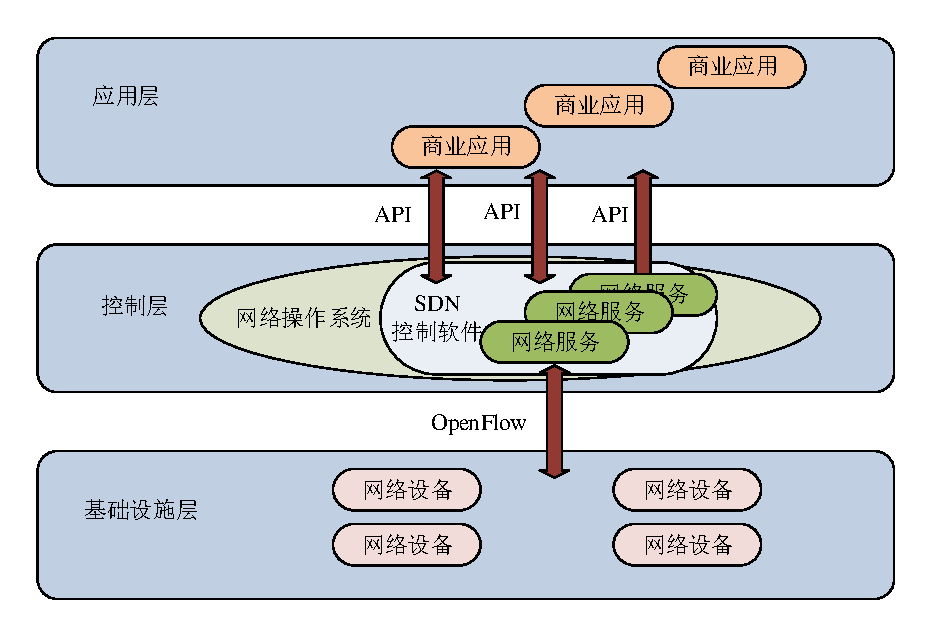
\includegraphics[width=0.7\textwidth]{logo/sdn}
  \caption{ONF定义的SDN三层架构图}
  \label{fig:sdn}
\end{figure}

传统网络设备紧耦合的构架在SDN体系中被拆分成应用、控制、转发三层分离的、可编程的开放构架。控制功能被转移到服务器(软件),上层应用、底层转发设施被抽象成多个逻辑实体。图\ref{fig:sdn}为ONF定义的SDN三层架构示意图\cite{SDN-2}。

应用层为网络各种应用需求,如移动视频、云存储、企业应用商店、桌面云、物联网等,通过北向接口灵活、可编程地调用控制层提供的网络抽象模型与业务功能。北向接口因为涉及业务较多,开放的标准化过程还处于研究阶段。

控制层为整个SDN构架的核心,也称为网络操作系统,可实现网络拓扑的集中控制和设备管理,进行流表的控制和下发。其主要功能包括路由优化、网络虚拟化、质量监控、拓扑管理、设备管理、接口适配等。

基础设施层包括标准化的网络设备和虚拟的网络设备,负责多级流表处理和高性能的数据转发,并作为硬件资源池,为控制层提供按需的网络拓扑、数据处理和数据转发。目前主流的网络设备和芯片产商已经提供了支持OpenFlow的网络设备。

南向接口定义了控制层与数据转发层(基础设施层)之间的交互协议,通过将转发过程抽象为流表,控制器可直接控制流表、屏蔽硬件,实现了网络虚拟化。物理硬件被淡化为资源池,可按需进行灵活分配和相互隔离。目前主流的控制层与转发层之间交互的协议为OpenFlow协议\cite{openflow-9}。
\subsection{OpenFlow协议}
OpenFlow协议\cite{openflow-5}是OpenFlow交换机和控制器之间交互信息的标准,也是OpenFlow交换机和控制器之间的接口标准。OpenFlow协议主要支持三种类型的消息:Controller-to-Switch消息,Asynchronous 消息和 Symmetric 消息\cite{openflow-6}。每种类型消息都有多个子类型。Controller-to-Switch消息由控制器发起直接管理和监视交换机状态,可能需要交换机做出响应;Asynchronous消息由交换机发起用于更新交换机的状态和控制器的网络事件;Symmetric消息可由控制器和交换机任一方发起。具体协议消息的类型及描述如下:

\begin{enumerate}
\item Controller-to-Switch消息
\begin{itemize}
\item Features:在建立传输层安全会话(Transport Layer Security Session)的时候,控制器发送feature请求消息给交换机,交换机需要应答自身支持的功能。一般在 OpenFlow 通道建立时使用。
\item Configuration:控制器设置或查询交换机上的配置信息。交换机仅需要应答查询消息。
\item Modify-state:控制器管理交换机流表项和端口状态等。
\item Read-state:控制器发送该消息来管理交换机状态。主要用于增加、删除或改变组/流表项和设置交换机端口属性。
\item Packet-out:控制器通过交换机指定端口发出网包。控制器按指定交换机端口发送数据包,并且转发经由Packet-in消息接收到的包。Packet-out消息必须包含完整包或一个指向存储在交换机中的完整包的缓冲区ID。该消息包含一系列按指定顺序执行的行为,若为空则丢弃该包。 
\item Barrier:控制器确保消息依赖满足,或接收完成操作的通知。
\end{itemize}
\item Asynchronous消息
\begin{itemize}
\item Packet-in:交换机收到一个网包,在流表中没有匹配项,则发送Packet-in 消息给控制器。如果交换机缓存足够多,网包被临时放在缓存中,网包的部分内容(默认128 字节)和在交换机缓存中的的序号也一同发给控制器;如果交换机缓存不足以存储网包,则将整个网包作为消息的附带内容发给控制器。
\item Flow-removed:交换机中的流表项因为超时或修改等原因被删除掉,会触发Flow-removed 消息,通知控制器删除流表。
\item Port-status:交换机端口状态发生变化时(例如down 掉),触发Port-status 消息。
\item Error:交换机发生问题时触发消息。
\end{itemize}
\item Symmetric消息
\begin{itemize}
\item Hello:交换机和控制器用来建立连接。
\item Echo:交换机和控制器均可以向对方发出Echo消息,接收者则需要回复Echo reply。该消息用来测量延迟、带宽、以及是否连接正常等。
\item Vendor:交换机提供额外的附加信息功能。为未来版本预留。
\end{itemize}
\end{enumerate}

OpenFlow协议的主要交互过程如下所示:

\begin{enumerate}
\item 控制器与交换机的连接建立:通过安全通道建立连接,所有流量都不经过交换机流表检查。当连接建立起来后,两边必须先发送OFPT\_HELLO消息给对方,该消息携带支持的最高协议版本号,接收方将采用双方都支持的最低协议版本进行通信。一旦发现共同支持的协议版本,则连接建立,否则发送OFPT\_ERROR消息,描述失败原因,并中断连接。
\item 控制器与交换机的连接中断:当连接发生异常时,交换机应尝试连接备份的控制器。当多次尝试均失败后,交换机将进入紧急模式,并重置所有的TCP连接。此时,所有包将匹配指定的紧急模式表项,其他所有正常表项将从流表中删除。此外,当交换机刚启动时,默认进入紧急模式。
\item 连接加密:安全通道采用\gls*{TLS}连接加密。当交换机启动时,尝试连接到控制器的TCP 6633端口。双方通过交换证书进行认证。因此,每个交换机至少需配置两个证书,一个是用来认证控制器,一个用来向控制器发出认证。
\item 流表项修改:该交互是核心交互过程,通过控制器下发的流表项修改指令完成。每条指令可能触发一系列OpenFlow协议消息,主要包括流表的增加、修改和删除。
\item 流表项移除:流表项的移出包括控制器主动模式和被动模式,控制器被动模式下,定时器计时结束:每个表项均有一个idle\_timeout定时器和一个hard\_timeout定时器(两者的计量单位都是秒),前者计算的是没有Flow匹配发生的时间,而后者则计算的是表项在流表中的总时间。一旦到达时间期限,交换机将自动删除该表项,同时发出一个流删除的消息;控制器主动模式下,控制器通过下发DELETE\_STRICT、 DELETE等指令相关的协议消息主动删除流表项
\end{enumerate}

\subsection{OpenFlow交换机}
OpenFlow交换机负责数据转发功能,主要技术细节由流表(flow table)、安全信道(secure channel)组成\cite{openflow-1},如图\ref{fig:of-switch}所示。

\begin{figure}[!htb]
  \centering
  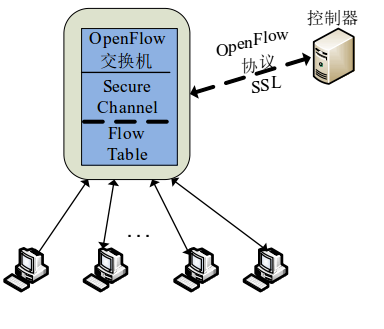
\includegraphics[width=0.7\textwidth]{logo/of-switch}
  \caption{OpenFlow交换机结构}
  \label{fig:of-switch}
\end{figure}

OpenFlow的转发策略主要保存在流表中,每个流表中都有很多表项(FlowEntry),这些表项可由外部控制器通过OpenFlow协议来写入、更新和删除。对于OpenFlow\ v1.3,每一个流表项都由匹配域、优先级、计数器、指令、超时以及Cookie组成\cite{openflow-8},如表\ref{table:flow}所示。当一个流进入交换机后,交换机会选择匹配的流表中优先级最高的一个执行相应的指令并更新计数器、超时等项。

\newcommand{\enter}[2][c]{%
  \begin{tabular}[#1]{@{}c@{}}#2\end{tabular}}
\begin{table}[!htb]
    \centering
	\caption{OpenFlow流表项结构}
	\label{table:flow}
	\begin{tabular}{|c|c|c|c|c|c|}
	\hline 
	\enter{匹配域 \\(Match Field)}& \enter{优先级 \\(Priority)}& \enter{计数器 \\(Counters)}& \enter{指令\\(Instructions)}&\enter{超时 \\(Timeouts)} & Cookie \\
	\hline
	\end{tabular}
\end{table}

匹配域用于进行对流的匹配。包括13个必须支持的域(Required):入端口、Ethernet目的地址、源地址、类型、IP协议号、IPv4源地址、目的地址、IPv6源地址、目的地址、TCP源地址、目的地址、UDP源地扯、目的地址。每一个域包含一个确定的值或者任意值(Any,表示任何值都能匹配),更准确的匹配可以用位掩码实现,但是每个域对掩码的支持与否不同。

优先级用于在流匹配到多个表项时的选择策略,这里优先级最高的被优先匹配。

计数器用于维护每个流表、每个流、每个队列等的统计数据,例如活动表项、包查找次数、包匹配次数、发送包数、接收字节数等。指令执行于匹配到的包,每个表项包括一系列指令,这些指令可能会直接对包进行改变,也可能改变行动集,或者管道处理。其中行动集是在包被转发前按照指定顺序执行的一系列行动,管道处理是包在各流表之间进行传递时,包与流表之间的互相作用关系。

超时机制用于交换机对于超时表项的自动删除,进而提高交换机的空间利用率。包括硬超时(指超过该值即删除,绝对时间)和软超时(指超过该值也没有匹配的流即删除,相对时间)。

匹配的具体过程如图\ref{fig:match}所示,具体流程如下。

\begin{enumerate}
\item 数据匹配字段从数据包中提取。用于表查找的数据包匹配字段依赖与数据包类型,这些类型通常包括各种数据包的报头字段,如以太网源地址或IPv4目的地址。除了通过数据包报头中进行匹配,也可以通过入口端口和元数据字段进行匹配。元数据可以用来在一个交换机的不同表里面传递信息。报文匹配字段表示报文的当前状态,如果在前一个表中使用Apply-Actions改变了数据包的报头,那么这些变化也会在数据包匹配字段中反映。 
\item 数据包匹配字段中的值用于查找匹配的流表项。如果流表项字段具有该值,它就可以匹配包头中的所有可能的值。如果交换机支持任意的的位掩码对特定的匹配字段,这些掩码可以更精确地进行匹配。优先级最高的流表项首先被匹配上,此时与选择流表项相关的计数器也会被更新,选定流表项的指令集也被执行。如果有多个匹配的流表项具有相同的最高的优先级的,所选择的流表项被确定为未定义表项\cite{openflow-7}。
\end{enumerate}

\begin{figure}[!htb]
  \centering
  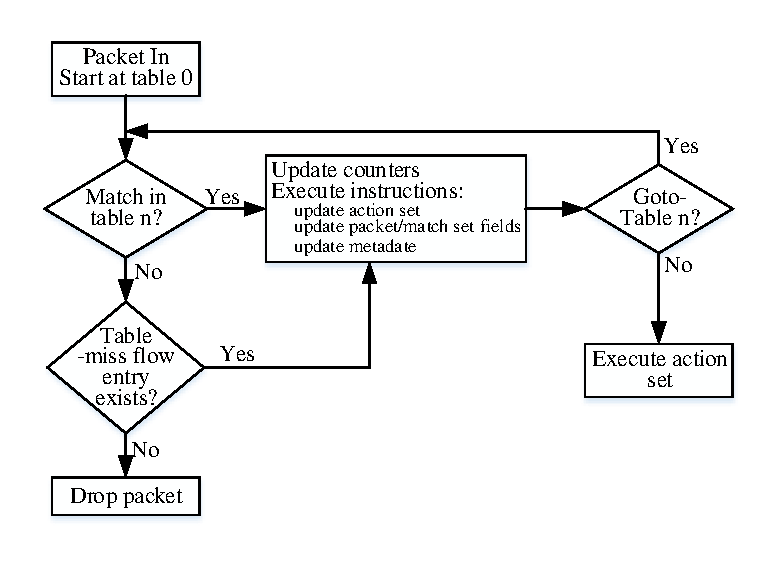
\includegraphics[width=0.7\textwidth]{logo/match}
  \caption{数据包匹配流程图}
  \label{fig:match}
\end{figure}

安全通道是连接OpenFlow交换机和控制器的接口,控制器通过这个接口,按照 OpenFlow协议规定的格式来配置和管理OpenFlow交换机,同时接收交换机传来的事件信息并发送数据包等。所有的OpenFlow通道信息必须用OpenFlow协议打包,OpenFlow通道通常用TLS来加密,但也能直接用TCP协议来实现。

目前,基于软件实现的 OpenFlow交换机主要有两个版本\cite{openflow-2},都部署于 Linux 系统:基于用户空间软件OpenFlow交换机操作简单,便于修改,但性能较差;基于内核空间的软件 OpenFlow 交换机\cite{openflow-3}速度较快,同时提供了虚拟化功能,使得每个虚拟机能够通过多个虚拟网卡传输流量,但实际的修改和操作过程较复杂。另外,斯坦福大学基于 NetFPGA 实现了硬件加速的线速 OpenFlow 交换机\cite{openflow-4},而网络硬件厂商如NEC、HP 等公司也已相继推出了支持 OpenFlow 标准的硬件交换机\cite{openflow-1}。
\subsection{OpenFlow控制器}
控制器是OpenFlow网络的核心部分,是整个网络的大脑,网络中所有的控制指令,数据流的转发操作都由它来完成,控制器中组件的好坏直接影响了整个网络的运行效率。


SDN控制器对网络的控制主要是通过南向接口协议实现,包括链路发现、拓扑管理、策略制定、表项下发等,其中链路发现和拓扑管理主要是控制其利用南向接口的上行通道对底层交换设备上报信息进行统一监控和统计,而策略制定和表项下发则是控制器利用南向接口的下行通道对网络设备进行统一控制。控制器负责控制其所管辖的OpenFlow交换机中的流表,包括流表内容的添加、修改以及删除等基本操作,操作的具体逻辑由控制器上运行的控制程序制定。网络使用者可以根据具体需求在控制器上编写控制程序,使得OpenFlow网络可以提供丰富的应用,体现了 OpenFlow网络的灵活性。在数据流处理的过程中,控制器的控制程序决定其所在网络中交换机上的流表内容。网路初始运行时,交换机上的流表为空,控制器必须具有全局网络视图, 如网络的拓扑结构、网络的当前运行状态等信息,才能针对不同数据流做出正确的决策。因此,控制器的设计是OpenFlow网络整体功能和效率的重点之一。

SDN北向接口是通过控制器向上层业务应用开放的接口\cite{SDN-4},其目标是使得业务应用能够便利地调用底层的网络资源和能力。通过北向接口,网络业务的开发者能以软件编程的形式调用各种网络资源;同时上层的网络资源管理系统可以通过控制器的北向接口全局把控整个网网络的资源状态,并对资源进行统一调度。因为北向接口是直接为业务应用服务的,因此其设计需要密切联系业务应用需求具有多样化的特征。同时,北向接口的设计是否合理、便捷,以便能被业务应用广泛调用,会直接影响到SDN控制器厂商的市场前景。

控制器负责整个SDN网络的集中化控制,对于把握全网资源视图、改善网络资源交付都具有非常重要的作用。但控制能力的集中化,也意味着控制器的安全性和性能成为全网的瓶颈;另外,单一的控制器也无法应对跨多个地域的SND网络问题,需要多个SDN控制器组成的分布式集群,以避免单一的控制器节点在可靠性、扩展性、性能方面的问题。
\section{网络虚拟化技术概述}
互联网不断地向前发展,必然会出现越来越多的应用和服务。然而现有的网络结构比较僵化,而且可扩展性很差,随着网络的发展,这些缺点日益突出,但是研发和部署新型的网络体系架构比较因难,难以更新,而且由于各个设备生产商自身利益的考虑,更加剧了这种困难。在这种背景下,网络虚拟化成为当前互联网面向未来网络体系架构过渡的一种有效解决方案,同时网络虚拟化也是未来网络体系架构应该具备的关键特性之一。

网络虚拟化技术\cite{Virtual-1},通过对共用的底层网络进行抽象并提供统一的可编程接口,将多个相互隔离且具有不同拓扑的虚拟网络映射到共用的基础设施上,为用户提供差异化服务。网络虚拟化允许多个租户占据相同的网络基础设施,每个租户会有一种错觉,认为可以对整个网络进行完整的处理。传统的网络虚拟化配置和操作都比较复杂,难以管理。原因就在于路由器和交换机变得越来越复杂,其配置操作的代价越来越大。而SDN的出现为网络虚拟化开启了另外一条道路,在SDN网络中,集中控制的优势使得对网络的管理变得灵活和高效。基于SDN的网络虚拟化是SDN思想的典型应用。本文选用OVX实现网络虚拟化模块,OVX通过给每个租户提供访问一个虚拟网络拓扑和一个完整的网络头空间来达到这样的目标,前者允许租户自定义拓扑结构,而后者保证功能性和流量隔离,即使不同的租户也可以选择重叠的寻址方案。OVX用作控制信道内的一个代理,呈现OpenFlow网络给租户,同时经由南向的OpenFlow接口控制底层的物理基础设施。通过暴露OpenFlow网络给租户,OVX允许租户使用自己的网络控制器控制自有的虚拟网络资源。换句话说,OVX基于同一底层物理网络创建多个vSDN网络,并且vSDN网络之间是相互隔离的,保证了租户虚拟网络的安全性。从底层网络的角度,OVX的表现为一个控制器,从租户的角度上看,OVX作为网络中具有OpenFlow能力的交换机集合\cite{OVX-2}。OVX具体的架构图如图\ref{fig:ovx}所示。

\begin{figure}[!htb]
  \centering
  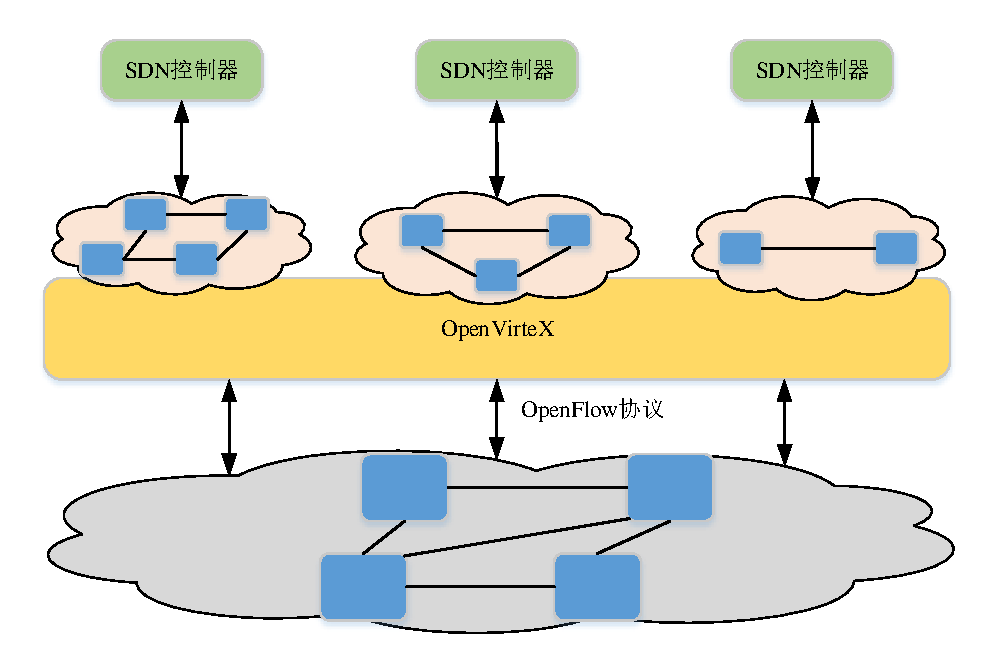
\includegraphics[width=0.7\textwidth]{logo/ovx}
  \caption{OVX网络虚拟化示意图}
  \label{fig:ovx}
\end{figure}

\section{OpenStack概述}

OpenStack是一个由NASA(美国国家航空航天局)和Rackspace合作研究并发起的,以Apache许可证授权的自由软件和开放源代码项目,主要为企业或者厂商提供了一种云服务的解决方案\cite{OpenStack-5}。OpenStack既可以被企业使用,在企业局域网内给员工提供私有云;也可以被厂商使用,进行二次开发,给云用户提供通过Internet访问的公有云服务。OpenStack通过一系列相关的服务提供IaaS解决方案。每个服务提供一个应用编程的API,这样有利于集成。管理员可以根据自己的需求安装部分或者全部服务\cite{OpenStack-6}。

\subsection{OpenStack架构}
OpenStack\ Juno版本的构架由9个服务组成,分别是Dashboard、Compute、Networking、Object Storage、Block Storage、Identity、Image Registry and Delivery Service、Telemetry和Orchestration\cite{OpenStack-4}。分别对应的各组件及各组件之间的协同关系如图\ref{fig:openstack}所示。

\begin{figure}[!htb]
  \centering
  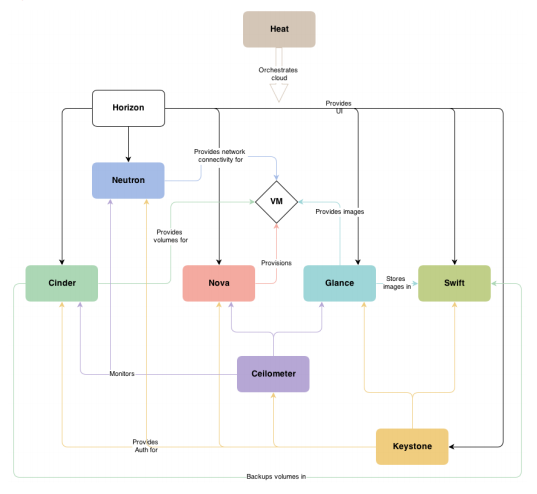
\includegraphics[width=0.7\textwidth]{logo/openstack}
  \caption{OpenStack概念架构图}
  \label{fig:openstack}
\end{figure}

主要组件的功能介绍如下\cite{OpenStack-3}。

\begin{enumerate}
\item Nova:计算服务是OpenStack的核心服务,它由nova-compute模块通过libvirt、XenAPI等管理hypervisor,从而管理虚拟机,此外它还通过nova-api服务向外提供如EC2兼容、管控功能等的接口,通过nova-scheduler模块提供虚拟机调度逻辑等,这些模块间的通信全部通过消息队列完成
\item Swift:对象存储服务是OpenStack最早期的两个服务之一(另一个是计算服务),在OpenStack平台中,任何的数据都是一个对象,swift-proxy模块对外提供如HTTP(S)、OpenStack Object API及与S3兼容的存取接口。对象的存取经swift-proxy接入后,还需要经三个模块进行定位,即account、container、object,这是因为在OpenStack中一个对象被描述为:某个帐户下某个容器中的某个对象。
\item Neutron:经过一定时间的演变,网络管理也抽离成一个独立的服务。在OpenStack的网络管理流程中,通常需要经过以下几个步骤:创建一个网络; 创建一个子网; 启动一个虚拟机,将一块网卡对接到指定的网络上;删除虚拟机;删除网络端口;删除网络。
\item Glance:Glance的出现是解决虚拟机镜像的管理问题,在生成一个镜像后,需要将镜像注册到系统的数据库中。当要实例化一个虚拟机时,需要将镜像分派到一台具体的实机上用来以启动虚拟机。因而Glance最重要的接口是镜像的注册和分派。
\item Cinder:Essex将nova的卷管理api独立化后,Folsom终于将卷管理服务抽离成了Cinder,Cinder管理所有的块存储设备,块设备可以挂接在虚拟机的实例中,然后虚拟机里的guest系统可以像操作本地卷一样操作块存储设备。Cinder需要处理的主要问题应该是接入各种块设备,如本地磁盘、LVM或各大广商提供的设备如EMC、NetApp、HP、华为,还有如Vmware提供的虚拟块设备等。
\item KeyStone:身份服务需要进行认证凭证的验证及关于用户、角色等信息,及所有相关的元数据,这些数据全都由Keystone服务管理,并提供CRUD的操作方法,另外这些信息可以从另一个认证服务中获取,例如使用LDAP做Keystone的后端。
\item Heat:Heat是一套业务流程平台,旨在帮助用户更轻松地配置以OpenStack为基础的云体系。利用Heat应用程序,开发人员能够在程序中使用模板以实现资源的自动化部署。Heat能够启动应用、创建虚拟机并自动处理整个流程。
\item Ceilometer:Ceilometer项目创建之初是为了实现一个能为计费系统采集数据的框架。社区后来更新了他们的目标,新目标是希望Ceilometer成为OpenStack里数据采集(监控数据、计费数据)的唯一基础设施,采集到的数据提供给监控、计费等项目使用。
\item Horizon:Horizon是一个用以管理、控制OpenStack服务的Web控制面板,它可以管理实例、镜像、创建密匙对,对实例添加卷、操作Swift容器等。除此之外,用户还可以在控制面板中使用终端(console)或VNC直接访问实例。
\end{enumerate}
\subsection{Neutron模块详解}
本文研究的主要内容,涉及最多的是OpenStack的Neutron模块,故本节对Neutron模块做详细的介绍,方便大家对论文的理解。

Neutron是OpenStack项目中负责提供网络服务的组件,它基于软件定义网络的思想,实现了网络虚拟化下的资源管理。在实现上充分利用了 Linux 系统上的各种网络相关的技术。一般的,OpenStack中网络实现包括VLAN、GRE、VXLAN等模式,本文中选取GRE模式搭建Neutron服务,GRE模式下的Neutron架构图如图\ref{fig:neutron}所示。

\begin{figure}[!htb]
  \centering
  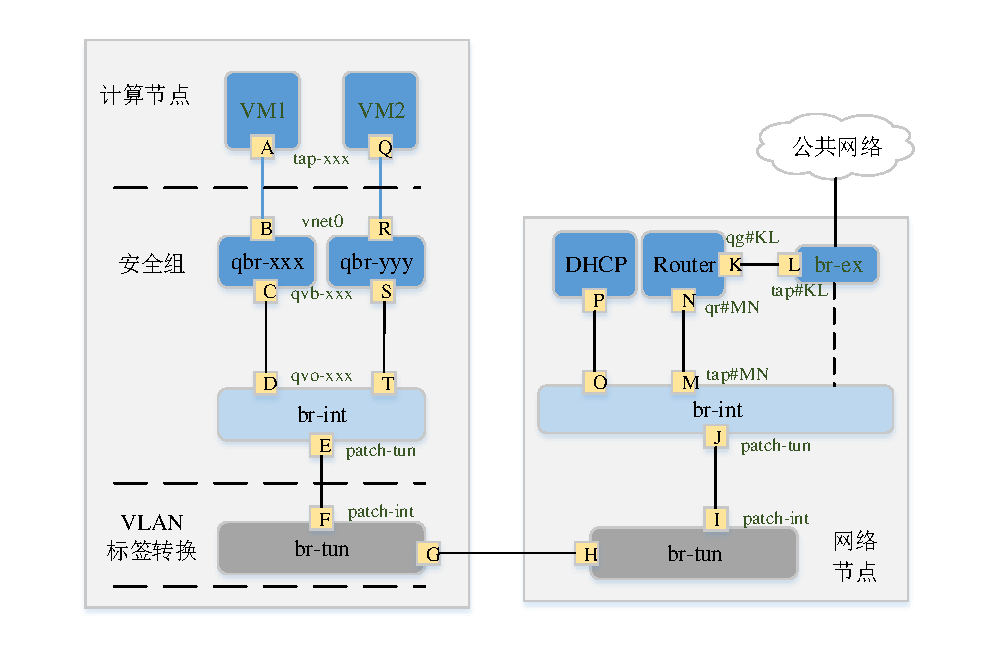
\includegraphics[width=0.7\textwidth]{logo/neutron}
  \caption{Neutron组件GRE模式架构图}
  \label{fig:neutron}
\end{figure}

在OpenStack中,所有网络有关的逻辑管理均在网络节点中实现,例如DNS、DHCP以及路由等。计算节点上只需要对所部属的虚拟机提供基本的网络功能支持,包括隔离不同租户的虚拟机和进行一些基本的安全策略管理(即安全组)。以抽象系统架构图为例,计算节点上包括两台虚拟机 VM1 和 VM2,分别经过一个网桥(如 qbr-XXX)连接到 br-int 网桥上。br-int 网桥再经过 br-tun 网桥(物理网络是 GRE 实现)连接到物理主机外部网络。网络节点上配置有DHCP、Router服务,对于访问外网的数据包,经由br-ex发出。各网桥功能及具体的服务如下所示。

\begin{enumerate}
\item qbr:在VM1中,虚拟机的网卡实际上连接到了物理机的一个TAP设备上(即 A,常见名称如 tap-XXX),A 则进一步通过VETH pair(A-B)连接到网桥 qbr-XXX 的端口 vnet0(端口 B)上,之后再通过 VETH pair(C-D)连到br-int网桥上。一般C的名字格式为 qvb-XXX,而 D 的名字格式为 qvo-XXX。注意它们的名称除了前缀外,后面的id都是一样的,表示位于同一个虚拟机网络到物理机网络的连接上。之所以 TAP 设备 A 没有直接连接到网桥br-int上,是因为 OpenStack 需要通过iptables实现安全组的功能。目前 openvswitch 并不支持应用iptables 规则的 Tap 设备。因为 qbr 的存在主要是为了辅助 iptables 来实现 security group功能,有时候也被
称为 安全网桥 。
\item br-int:br-int是一个openvswitch网桥。br-int 在 GRE 模式中作为一个 NORMAL 交换机使用,因此有效规则只有一条正常转发。如果两个在同一主机上的 vm 属于同一个 tenant 的(同一个 vlan tag),则它们之间的通信只需要经过 br-int 即可。在网络节点上,该网桥上挂载了很多进程来提供网络服务,包括路由器、DHCP服务器等。这些进程不同的租户可能都需要,彼此的地址空间可能冲突,也可能跟物理网络的地址空间冲突,因此都运行在独立的网络名字空间中。 
\item br-tun:br-tun将带有 vlan tag 的 vm 跟外部通信的流量转换到对应的 gre 隧道,这上面要
实现主要的转换逻辑,规则要复杂,一般通过多张表来实现。这些规则组成的整体转发逻辑如图\ref{fig:br-tun}所示。其中patch-int(即端口F)是连接到br-int上的VETH pair的端口,gre端口(即端口G),对应vm到外面的隧道。所有到达br-tun的网包,均交给Table0,如果该数据包来自gre端口,即从外部服务器发送至此,则交给Table2进一步处理;如果该数据包来自patch-int端口,即从服务器内部发出,目的主机位于服务器之外,则交给Table1进行下一步的处理,否则丢弃该包。Table2主要实现了tunnel号向vlan号的转换;Table10主要实现了反向规则的添加,Table20和Table21主要实现了vlan号向tunnel号的转换,两者的区别在于,Table20主要针对单播,而Table21主要针对多播/组播。

\begin{figure}[!htb]
  \centering
  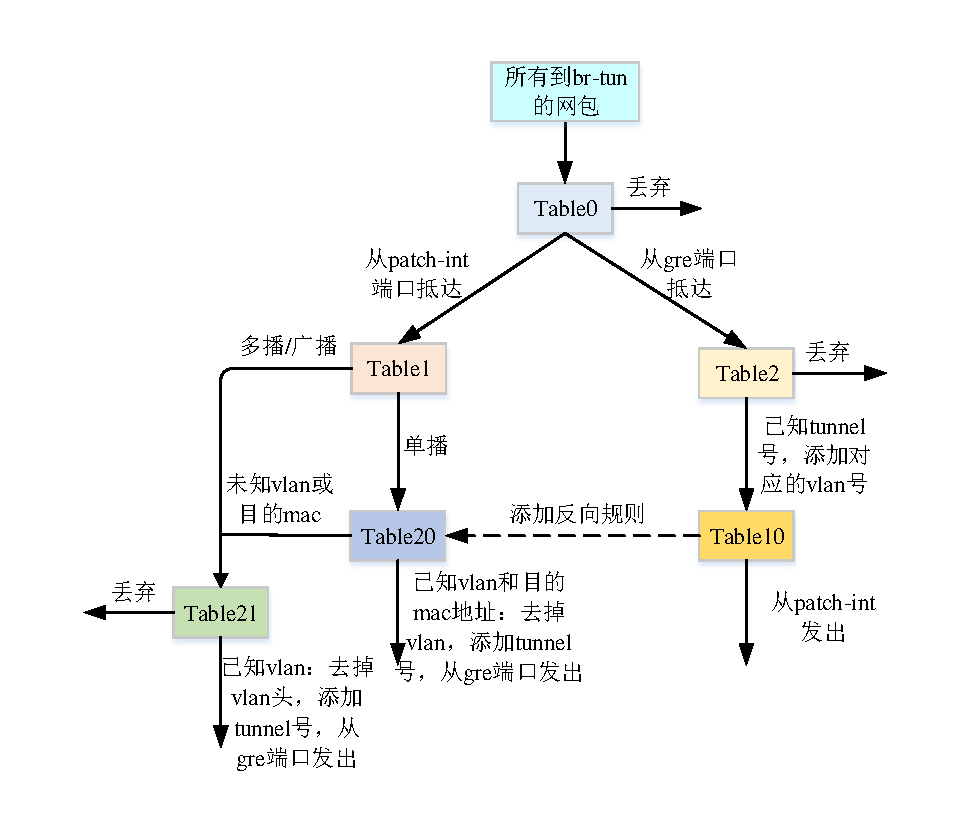
\includegraphics[width=0.7\textwidth]{logo/br-tun}
  \caption{br-tun网桥转发规则}
  \label{fig:br-tun}
\end{figure}

\item br-ex:br-ex直接连接到外部物理网络,一般情况下网关在物理网络中已经存在,则直接转发即可。如果对外部网络的网关地址配置到了br-ex(即br-ex作为一个网关),需要将内部虚拟机发出的流量进行SNAT,之后发出。
\item dhcp 服务:dhcp 服务是通过 dnsmasq 进程(轻量级服务器,可以提供 dns、dhcp、tftp 等服务)来实现的,该进程绑定到 dhcp 名字空间中的 br-int 的接口上。可以查看相关的进程。
\item router服务:首先,要理解什么是 router,router 是提供跨 subnet 的互联功能的。比如用户的内
部网络中主机想要访问外部互联网的地址,就需要 router 来转发(因此,所有跟外部网络的流量都必须经过 router)。目前 router 的实现是通过 iptables 进行的。 同样的,router 服务也运行在自己的名字空间中。防火墙服务就是在router命名空间中实现。默认情况,访问外部网络的时候,数据包会从 qg-xxx 端口发出,经过 br-ex 发布到外网。外网访问租户内网的时候,会从 qr-xxx 端口发出,发给br-int。

\end{enumerate}

\section{本章小结}
本章主要介绍了SDN、网络虚拟化及OpenStack的相关技术。重点介绍了OpenFlow协议,OpenFlow交换机的组成以及OpenFlow流表主要字段以及流表匹配过程。对于网络虚拟化技术,由于本文需要实现SDN模式下的网络虚拟化,所以仅对适用于本文的SDN模式下的网络虚拟化技术做了简单的概括。随后介绍了OpenStack的模块构成,而对于本文用到的Neutron模块,进行了详细的架构剖析。本文的系统架构,主要在以上各部分的基础上,进行集成开发。后续会对整体的系统架构做详细的介绍。
\chapter{基于SDN的云平台架构设计}
基于SDN的云平台多租户虚拟网络定制化的研究,主要是将SDN集中控制和可编程的优势,集成到云数据中心,通过网络虚拟化技术,为租户提供相互隔离的vSDN网络,vSDN网络由租户自有的控制器实现集中管控。物理网络的集中管控,方便运营商对数据中心网络的管理和维护;租户vSDN网络的集中管控,便于租户利用控制器开发适合自己的上层应用。本章主要对系统架构进行详细介绍。
\section{关键技术分析}
\subsection{需求分析}
基于SDN的云平台多租户虚拟网络定制化的实现,首先解决的是物理网络资源的虚拟化,其次是在虚拟化的基础上进行虚拟网络的带宽时延测量,随后根据测量数据进行链路的定制化,最后为方便用户的操作,完成前端Web界面的设计与实现。系统的整体需求如图\ref{fig:demand}所示。

\begin{figure}[!htb]
  \centering
  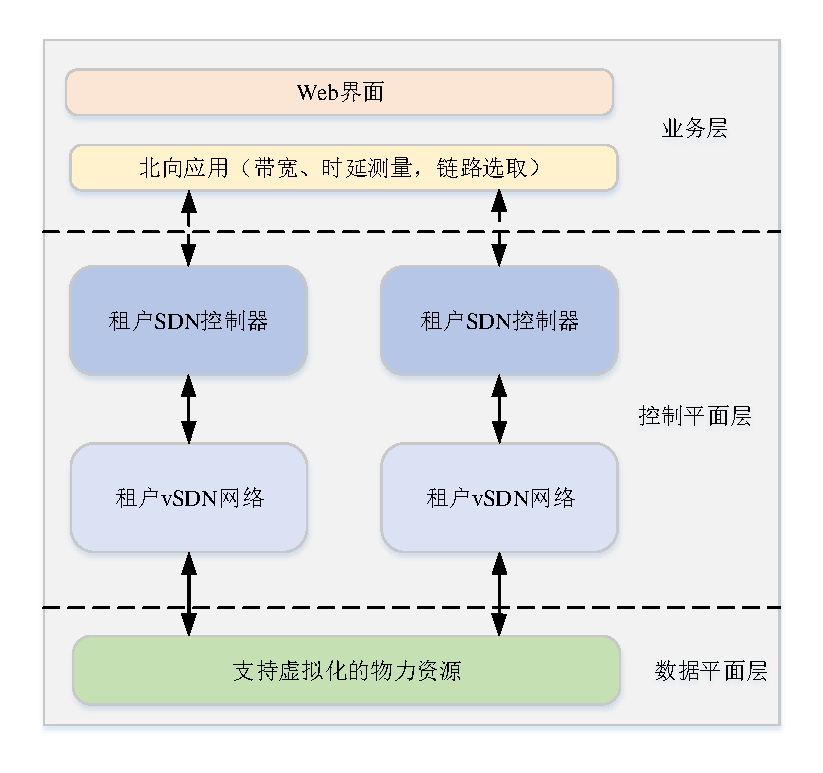
\includegraphics[width=0.7\textwidth]{logo/demand}
  \caption{系统需求分析图}
  \label{fig:demand}
\end{figure}

网络虚拟化,需要实现物理资源的隔离,以此同时,还要满足虚拟网络支持SDN模式,本文选用支持资源虚拟化的SDN控制器来完成该功能,通过对底层物理网络下发的流表,添加租户ID等相关信息,完成底层网络中租户隔的离工作。通过自身维护物理网络与虚拟网络的映射表,为上层SDN交换机提供支持OpenFlow协议的虚拟网络,此时租户便可利用自身的SDN控制器完成对vSDN网络的集中管控,进而实现自有的定制化操控。

在虚拟资源之上进行链路带宽时延等信息的测量工作,需要实现SDN模式下链路带宽、时延的精确测量,由于SDN的集中控制和可编程的先天优势,控制器端可以看到全局的网络拓扑,与此同时,OpenFlow协议的规范性和便捷性,方便了我们实现可用带宽、已用带宽、时延的精确测量工作,测量的数据成为用户做出决策的考量值。

链路的定制化,需要用户根据链路的时延、带宽等信息,选取便于传输的最优链路,通过定制化流表的下发,租户便可以对数据中心的虚拟机,自定义数据的传输路径。

前端的Web界面方便了用户的操作,用户可以在web界面,完成对数据中心网络的定制化操作。包括物理、虚拟网络的拓扑获取,链路带宽、时延的前端展示,虚拟网络的创建,定制化链路的前端选取等功能。一系列的操作,需要实现租户之间的隔离,为此我们需要添加认证模块,对租户的请求进行认证解析。实现租户操作的安全性和隔离性。

\subsection{关键技术}
本文旨在构建一个基于SDN的多租户虚拟网络定制化的云平台,该平台一方面实现对数据中心网络的集中控制,方便运营商对数据中心网路的管理和运维,加快新业务的引入速度,运营商可以通过可控的软件部署相关的功能,该自动化部署和运维故障诊断,减少了网络的人工干预,降低了网络的运营费用,也降低了出错率。与此同时,通过虚拟化技术,基于底层的统一物理资源,虚拟出相互隔离的租户vSDN网络,vSDN网络由租户自己的SDN控制器实现集中管控,方便租户的自定义操控,同时,租户可以为自己的控制器开发特有的北向应用,从而定制化数据中心业务需求,当然租户对数据中心虚拟网络的集中控制,便于租户实现对自有网络的监控工作,并可根据当前网络负载定制化链路的转发路径,实现数据包的最优化传输。为实现上述功能,需要突破以下关键技术。

\begin{enumerate}
\item 基于SDN的云平台系统搭建。将SDN集成到云平台数据中心,系统的搭建尤为重要,如何在实现相应功能,满足租户需求的情况下,搭建一套性能稳定的系统成为本文的关键所在。为此,本文创新性地提出了基于SDN的云平台多租户虚拟网络定制化机制,在实现对数据中心网路集中控制的同时,利用虚拟化技术虚拟出相互隔离的vSDN网络,该网路由租户自有的控制器实现集中管控,这样,租户便可以利用自己的SDN控制器完成对自有网络的灵活控制。为方便与OpenStack云平台的集成,本文在对OpenStack云平台改动最小、性能降低最低的情况下,完成了整体系统的搭建,系统的虚拟化平台与OpenStack网络模块Neutron分工合作,Neutron主要负责OpenStack内部网络资源的管理和控制,而本文中支持SDN模式的虚拟化平台主要负责物理服务器之间的SDN网络的管理和控制,两者协同合作,共同完成SDN与OpenStack的集成工作,开放控制器给租户,实现租户对数据中心虚拟网络的灵活管控。
\item 链路带宽、时延的测量。SDN控制器开放给租户后,利用SDN控制器实现对vSDN网络负载的精确测量,是每一个租户希望看到的,测量数据的精确性,直接决定了数据转发策略制定的合理性。因此,全局网络的带宽、时延数据的测量,在本文中起到关键作用。针对带宽、时延,本文创新性地提出了SDN模式下的测量方法。首先针对链路可用带宽,本文采用包对技术,精确地测量了链路的可用带宽,测试证明,该方法在低带宽模式下具有精确的测量结果。针对时延,本文基于三角架构,通过统计数据包的传输时间差,完成了时延的精确测量。带宽和时延数据,成为了租户进行链路定制化的重要依据,租户根据当前链路的负载情况,可以选取一条最优的链路进行数据传输,在提高云平台数据中心带宽利用率的同时,极大地提高了租户网络的数据传输速率。
\end{enumerate}

\section{系统架构设计}
\subsection{系统总体设计图}
系统主要由5个模块组成。分别为底层网络资源和计算资源模块、网络虚拟化模块、控制器模块、通信模块和GUI模块。总体的架构图如图\ref{fig:artic}所示。

\begin{figure}[!htb]
  \centering
  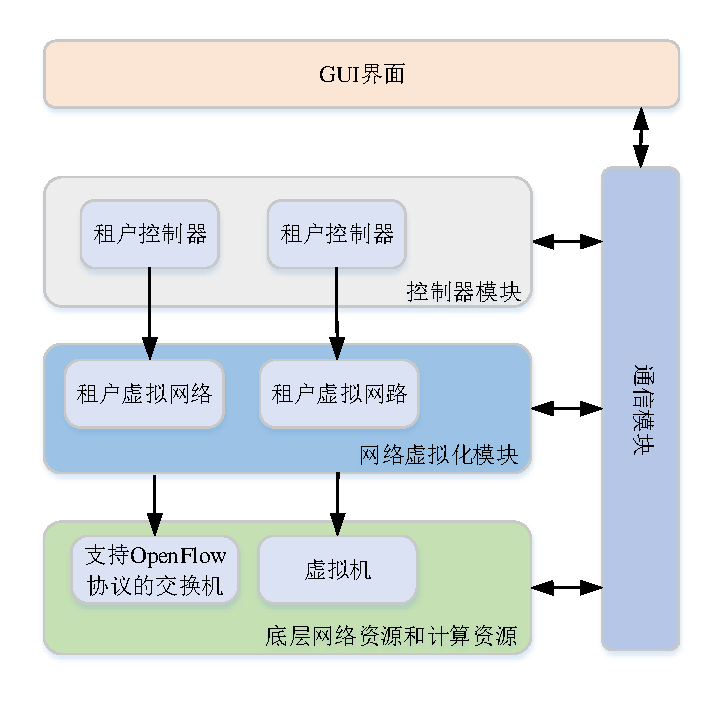
\includegraphics[scale=0.8]{logo/architecture-a}
  \caption{系统整体架构图}
  \label{fig:artic}
\end{figure}

从图中可以看出,架构底层主要包含支持OpenFlow协议的交换机,以及OpenStack内部的虚拟机资源,交换机既包含OpenStack内部的虚拟网桥,亦包含连接物理服务器之间的OpenFlow交换机,将这部分网络开放给租户,主要是为了便于租户实现对数据中心物理网络的可控性。租户可以根据链路时延、带宽定制化最优数据传输链路。网络虚拟化模块,本文基于支持网络虚拟化的SDN控制器实现,一方面实现对底层网络和计算资源的集中控制。另一方面,可以创建相互隔离的租户虚拟网络,该虚拟网络支持SDN模式,租户可利用控制器实现对虚拟网络的集中管控。自主开发北向应用,实现特有的功能。

控制器模块主要实现对租户控制器的管理。租户控制器实现对自有vSDN网络的集中管控,该控制器运行于特定虚拟机之中,租户可以登录虚拟机,进行相应的配置和开发工作。每一个vSDN网络对应唯一的SDN控制器。现有的控制器镜像,已经为其开发了进行链路带宽、时延测量的北向应用。

通信模块主要实现进程间的异步通信,所涉及到的功能有,前端对网络拓扑的获取、带宽时延数据的获取以及虚拟网络创建请求的下发,这一系列的功能均通过通信模块,分别和控制器、网络虚拟化模块完成数据的交互。

前端GUI界面,主要为了方便用户的操作,用户可以在其Web界面,通过最直接方式,完成对数据中心网络的定制化操作。主要包括网络拓扑的显示,链路带宽、时延的前端展示,虚拟网络的创建操作,定制化链路的前端选取等功能。前端模块的实现极大地提高了用户体验效果。

\subsection{系统详细架构图}
在OpenStack云平台数据中心网络中采用SDN架构,核心思想是用控制器对网路运营模式实现统一管控。现有云数据中心网络的模式均为单一节点控制,该模式下的SDN网络对于租户是不可见的。本文提出了多租户虚拟化网络的定制和管理方案,实现了租户自有控制器对虚拟网络的灵活控制。多租户对应多控制器的机制便于租户对自有网络进行带宽时延查询、定制化流表下发、链路切换、控制器北向接口开发实验等自定义操作。系统的详细架构图如图\ref{fig:architecture}所示。

\begin{figure}[!htb]
  \centering
  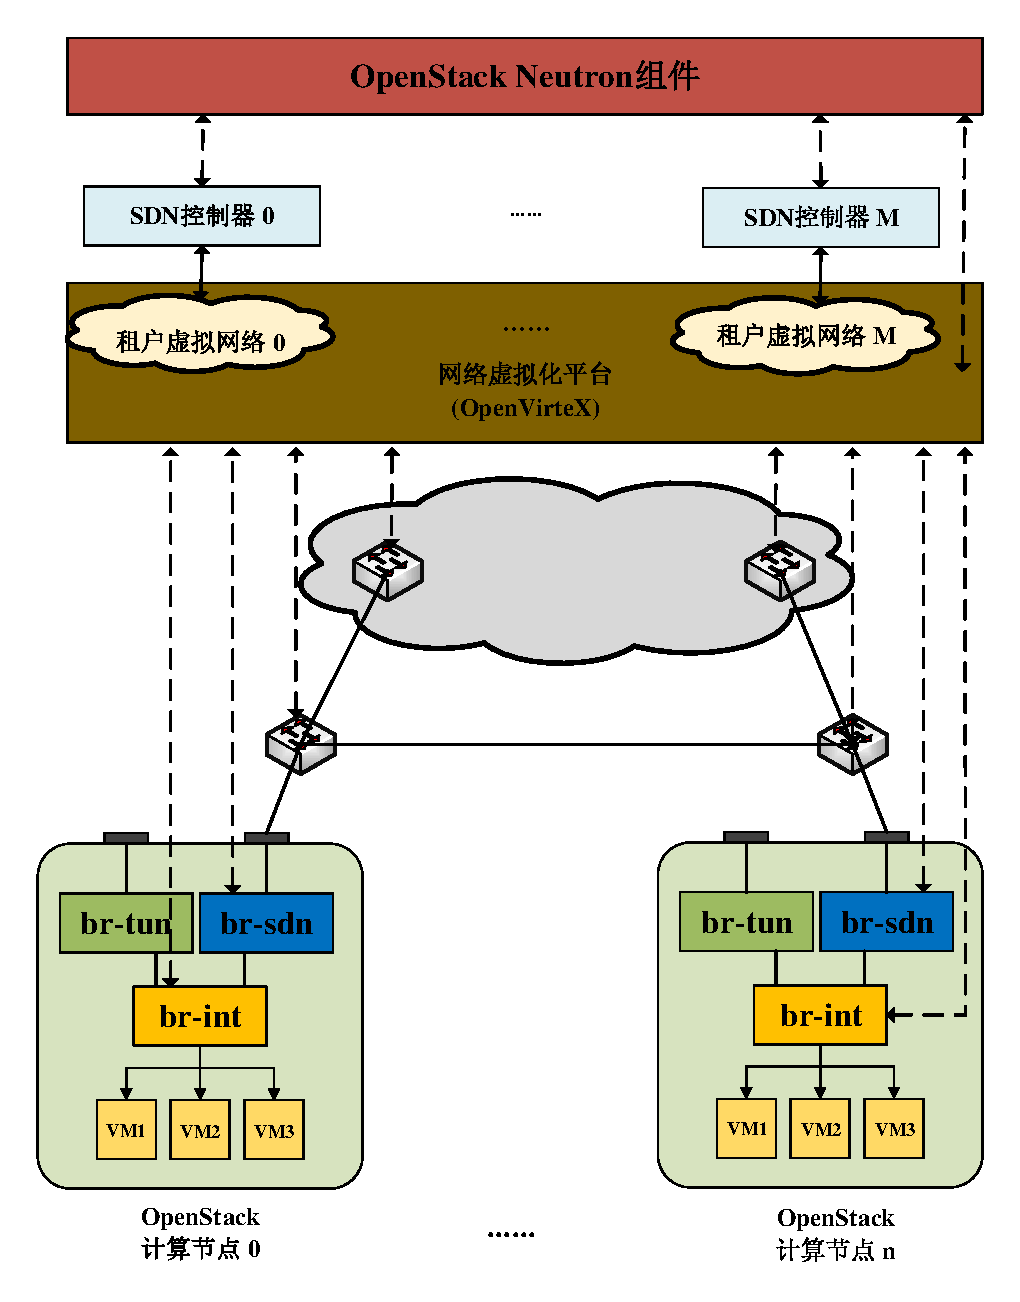
\includegraphics[width=0.7\textwidth]{logo/architecture}
  \caption{系统详细架构图}
  \label{fig:architecture}
\end{figure}

在兼容现有OpenStack网络模式的前提下,为OpenStack平台的每个计算节点添加br-sdn网桥,由于br-int网桥实际就是一个NORMAL交换机,不管其受SDN控制器控制与否,不会影响其作用,故我们将该网桥以及连接物理服务器之间的支持OpenFlow协议的交换机均受OVX控制器进行管控,OVX控制器实现对网络的集中控制,与此同时,OVX支持SDN模式下的网络虚拟化,可以虚拟出相互隔离的vSDN网络,vSDN网络由租户自己的控制器进行集中控制。前端GUI模块基于OpenStack的Horizon模块进行二次开发,为其添加两个Panel,分别实现对物理网络和虚拟网络的拓扑展示,全局链路带宽、时延展示,以及虚拟网络创建和删除的前端操作。

在该架构图中,OVX与OpenStack中的Neutron组件并列存在,Neutron主要管控OpenStack内部的虚拟网络,包括各种防火墙、Router、DNS服务,而OVX主要负责连接服务器之间的物理网络的管理,两者并列存在。相互协同工作。这种实现模式可以在对OpenStack云平台改动最小、性能影响最低的情况下完成SDN与OpenStack的集成。

对于数据传输,现有架构下,有两种模式可以选择。租户可以选择使用传统网络模式进行数据的传输,数据经br-int和br-tun,由传统模式交换机,进行数据的传输。与此同时,租户亦可通过流表的下发,实现SDN模式下的数据传输,该模式下,数据经由br-int和br-sdn,途径支持OpenFlow协议的交换机,完成数据的转发工作。两种模式的并存,租户可以自主选择切换模式。现有的SDN模式,相比于传统模式,SDN模式下租户可以开发自己的北向应用,实现数据中心网络特定功能的开发。当然SDN现有模式仅仅实现了二层转发,跨路由的传输现阶段只能通过传统模式实现。

\subsection{系统流程图}
系统的整体流程图如图\ref{fig:workflow}所示。流程图主要对系统整体的工作流进行了阐述。详细讲解了从虚拟网络创建到链路定制化的整个流程。

\begin{figure}[!htb]
  \centering
  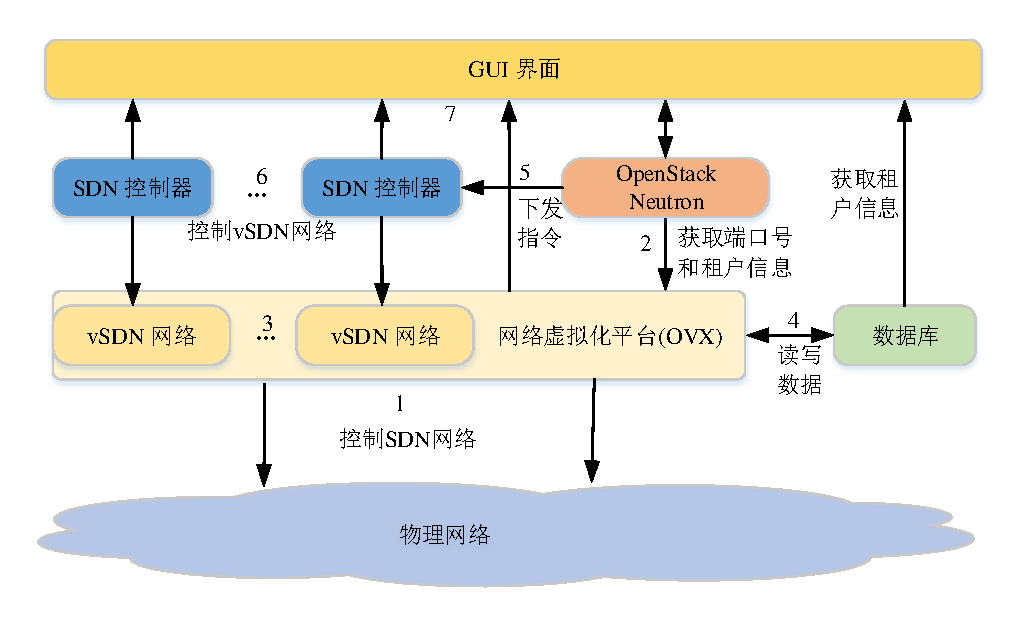
\includegraphics[width=0.7\textwidth]{logo/workflow}
  \caption{系统流程图}
  \label{fig:workflow}
\end{figure}

\begin{enumerate}
\item 网络虚拟化平台OVX实现对底层物理网络管理,完成物理网络的集中控制。本研究为其开发了创建虚拟网络的API接口\emph{createCustomNetwork},租户可以调用该接口,实现虚拟网络的创建。OVX自身维护虚拟网络与物理网络的映射表,完成南北向指令的映射工作。
\item 从OpenStack Neutron侧,获取虚拟机以及虚拟机绑定br-int网桥的端口信息,OVX本身只能获取到交换机的连接信息,两者结合,得到全网的完整拓扑信息图。基于此物理网络信息,进行虚拟网路的创建。
\item 本研究对OVX封装了创建虚拟网路的\emph{createCustomNetwork}接口,调用该API接口,完成虚拟网络的创建。该虚拟网络基于底层的物理资源,可以是底层物理资源的同构子图,也可以是自定义的虚拟网络拓扑图。
\item 在网络虚拟化平台OVX侧,每个虚拟网络由\emph{virtualnetworkid}进行标识。在OpenStack中,每个租户有自己的ID号\emph{tenantid}。本文将两者的对应关系存储到数据库中。另外,对创建的虚拟网络以及虚拟网络和物理网络的对应关系,亦存储到数据库中,方便用户进行数据的读取和修改。本研究采用MongoDB数据库完成上述操作。由于MongoDB为非关系型数据库,该数据库釆
用BSON语法格式存储数据,可以实现对海量数据的存储管理,它的特点是高性能、易部署和易使用,非常适合存储大数据\cite{mongodb}。

\item OpenStack Neutron侧发送指令到SDN控制器。现阶段,指令主要包括带宽/延迟测量以及定制化流表的下发。未来我们的平台将提供更多的功能。
\item SDN控制器接收到消息,通过我们开发的应用,完成相应的测量工作。最后返回对应的结果。租户可以登录到SDN控制器所在的虚拟机,开发自己的应用程序,以实现更多的功能。
\item GUI界面完成物理网络、虚拟网络、链路带宽、时延等信息的获取,在前端界面完成展示工作。
\end{enumerate}

\section{模块详解}
\subsection{网络虚拟化模块}
网络虚拟化允许租户共用底层的基础设施资源,通过逻辑的隔离,租户只能访问自有的虚拟网络,以确保租户通信的安全性。通过虚拟化技术,可以在单一物理资源之上创建相互隔离的用户组,并且该用户组在网络中保持极高的可扩展性和安全性。网络虚拟化技术可以提高数据中心的运行效率,加速业务的部署。提供更为便捷的业务更新。

本文选用的网络虚拟化平台,通过为每个租户提供一个可访问的虚拟网络拓扑和一个完整的网络头空间来完成虚拟网络的创建,呈现OpenFlow网络给租户,同时经由南向的OpenFlow接口控制底层的物理基础设施,完整的网络头空间保证了租户虚拟网络功能性和流量隔离\cite{Virtual-3}。与传统网络切片进行虚拟化相比,该模式允许不通租户使用相同的网络属性(诸如:IP、TCP/UDP端口等),而且,网络切片所创建的虚拟网络必须是物理网络的同构子图,租户不可以自定义虚拟网络拓扑图。网络虚拟化平台在北向租户看来为支持SDN架构的交换机集合,在南向基础物理设施看来,为SDN控制器。网络虚拟化模块主要由四部分组成,分别为面向网络的南向接口、面向租户的北向接口、全局映射表和API服务器\cite{OVX-1}。具体架构如图\ref{fig:virtual}所示。

\begin{figure}[!htb]
  \centering
  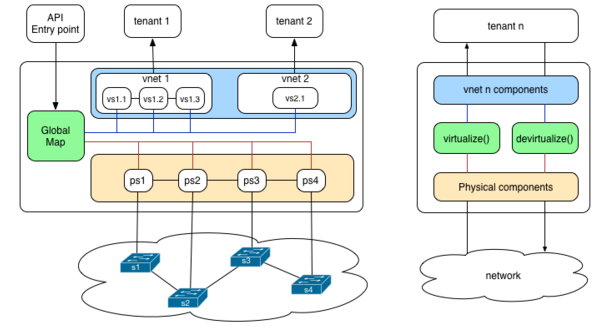
\includegraphics[width=0.7\textwidth]{logo/virtual-detail}
  \caption{网络虚拟化模块架构}
  \label{fig:virtual}
\end{figure}

面向OpenFlow网络的南向接口,连接底层基础设施,管理虚拟平台和基础设施之间的通信信道。面向租户的北向接口,呈现vSDN网络给租户,管理租户SDN控制器和vSDN网络之间的通信信道。全局映射表,用于存储物理网络与虚拟网络拓扑的对应关系,并且分别通过南、北向接口连接这两个网络。API服务器,主要用于监听JsonRPC调用,对用户请求作出相应的处理。

虚拟化平台通过南向OpenFlow信道实现与底层物理网络通信,对于底层网络拓扑,虚拟化平台通过定时发送LLDP报文实现链路的探测,最终获取到整个物理网络的拓扑信息。而对于租户vSDN网络,租户控制器下发的LLDP报文,并未直接发送至底层OpenFlow交换机,而是被虚拟化平台接收,虚拟化平台模拟LLDP的整个过程,将租户vSDN网络的拓扑信息告知租户控制器,从而实现租户控制器对vSDN网络的探测。从南向看来,虚拟化平台被看作是SDN控制器,实现对底层OpenFlow网络的集中控制;从北向租户控制器看来,虚拟化平台为支持OpenFlow协议的交换机集合。在图\ref{fig:virtual}中,北向接口开放给租户,而南向接口通过OpenFlow信道实现对底层网络的管控,两者互不可见,通过映射模块建立起对应关系。北向租户控制器消息的下发和南向物理交换机消息的上传均通过查询映射表修改的方式,完成数据的翻译过程。如图\ref{fig:virtual}右侧所示,北向租户控制器消息通过devirtualize()进行去虚拟化处理,而南向交换机消息通过virtualize()进行虚拟化处理。

虚拟化平台中的租户隔离,作为虚拟化的一个核心需求,本研究中通过在MAC字段中添加额外的信息,使不同租户的流量得到隔离。具体来讲,虚拟化平台在对底层SDN网络下发定制化流表,使得数据包进入边缘交换机时,对数据包的MAC地址做了修改,添加了流ID、租户ID、虚拟链路ID。流ID主要用于查询流入虚拟链路的特定流表;租户ID实现不同租户的隔离;虚拟链路ID用于跟踪这条虚拟链路。当数据包传输至目的边缘交换机时,虚拟化平台下发特定流表,将数据包中的MAC地址字段修改为原始地址,数据包顺利到达目的主机。

综上所述,本文中选用的虚拟化平台主要实现以下四个功能。
\begin{itemize}
\item 创建了一个特定拓扑的独立虚拟网络。
\item 租户使用自己的控制器对虚拟网络进行集中控制。
\item 为每个租户使用整个地址空间,租户虚拟网络可以使用相同的IP地址
\item 可以动态地改变运行中的虚拟网络,并且能够在物理失效的情况下,自动恢复。
\end{itemize}


\subsection{通信模块}
通信模块基于消息队列实现,消息队列是一种应用程序与应用程序之间的通信方式。应用程序通过读写队列中的消息来完成相互的通信。消息传递指的是程序之间通过在消息中发送数据进行通信,而不是通过直接调用彼此来通信。队列作为一个消息代理,为应用程序提供用于存储发送或者接受消息的平台。直到消息从队列中被接收端读取为止。具体的通信模块如图\ref{fig:rabbitmq}所示。

\begin{figure}[!htb]
  \centering
  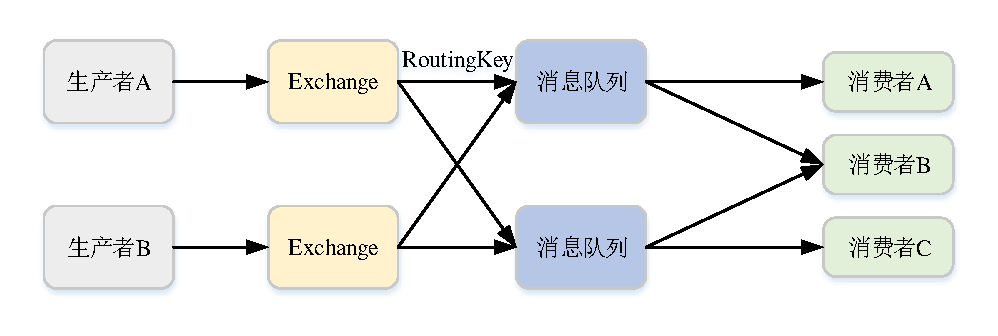
\includegraphics[width=0.7\textwidth]{logo/rabbitmq}
  \caption{通信模块架构图}
  \label{fig:rabbitmq}
\end{figure}

由图中可以看出,生产者绑定Exchange,Exchange是一个消息交换机,它指定消息按什么规则,路由到哪个队列。具体的路由规则由RoutingKey设定,RoutingKey作为路由关键字,Exchange根据这个关键字进行消息投递。队列用于消息的存储,直到消息被消费者从队列中读取完毕\cite{rabbitmq}。

本文基于消息队列实现通信模块,带来诸多好处。首先消息队列具有可持久性,即使接受方未启动,队列中的消息仍然存在,待接收端启动后,继续从消息队列中读取消息,这种允许延后处理消息的能力极大地提高了通信模块的健壮性。与此同时,消息队列的“只送达一次”和“只处理一次”保证了消息处理的安全性。

\subsection{控制器模块}
控制器作为中间桥梁,连接北向应用和底层的OpenFlow网络设备,一方面,SDN控制器实现对底层网络的集中管控,通过南向接口完成流表的下发。控制器的集中控制可以完成对底层网络的状态监控、转发策略制定以及流量调度等功能;另一方面,控制器开放北向可编程接口给用户,用户可以从实际出发,编写特定的应用程序,自定义网络策略。

本研究中,我们提供了基于Ryu控制器的Linux镜像,租户可以基于此镜像进行控制器的创建,租户只需要将自己创建的虚拟网络指向自己的SDN控制器,即可利用自有的控制器实现对虚拟网络的集中控制。租户可以根据自身需求进行控制器北向应用的相关开发工作。本文主要实现了链路时延、带宽的测量,以及定制化流表的下发实验。

本文选用的Ryu控制器,是由日本最大的电信服务提供商NTT主导幵发的基于Python语言的开源控制器,Ryu控制器为用户提供了丰富的API接口,便于开发人员创建新的应用程序,Ryu架构及主要组件如图\ref{fig:ryu}所示\cite{Ryu-1}。协议支持组件主要提供了对各种网络协议的支持,比如:Netconf,OpenFlow, OF-config等;库文件提供了各种版本的OpenFlow协议标准;内置应用提供了必要的网络功能,基于此,用户可以开发出更多定制化的应用程序;REST组件主要为用户提供丰富的北向API接口。

\begin{figure}[!htb]
  \centering
  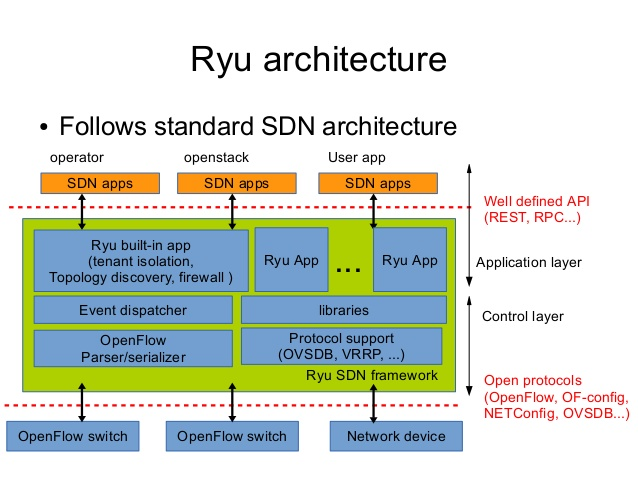
\includegraphics[width=0.7\textwidth]{logo/ryu}
  \caption{Ryu架构图}
  \label{fig:ryu}
\end{figure}

\subsection{GUI模块}
为方便用户对虚拟网络的操作,本研究为用户开放了前端GUI接口,用户可以在前端实现物理网络、虚拟网络的拓扑获取,虚拟网络的创建和删除,全局网络带宽、时延的测量,以及数据传输链路的选取等操作。开放的GUI界面,可以在用户不理解底层实现的基础上,进行便捷行的操作。

针对GUI模块,本文基于OpenStack的Horizon模块进行二次开发,为其添加了物理网络和虚拟网络显示的模块,在显示拓扑的基础上,实现虚拟网络创建、删除,以及网络负载查询等功能。

为了租户请求的安全性,我们为其添加了认证机制,在租户发出某一请求时,首先会通过自己的用户名和密码向认证模块申请token,认证成功后,会返回该用户的唯一token标识,token中包含租户的基本信息,以及租户的权限信息,如果认证失败,该次请求结束,并返回错误信息。如果成功,租户会将刚才的请求与现有的token值合并,再一次发送至后端服务器进行请求,服务器端对token验证成功后,执行相应的请求,并将请求结果返回给前端。具体的流程如图\ref{fig:credentials}所示。

\begin{figure}[!htb]
  \centering
  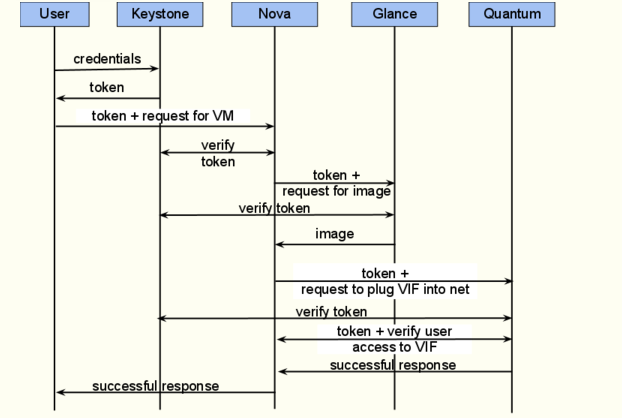
\includegraphics[width=0.7\textwidth]{logo/credentials}
  \caption{请求认证图}
  \label{fig:credentials}
\end{figure}

\section{本章小结}
本章主要对系统的架构做了详细的说明,为后面系统功能的实现做了铺垫。首先论文介绍了需求分析和关键技术,对本文研究内容的需求做了简要阐述,介绍了网络虚拟化、链路负载测量、链路定制化、前端Web界面的简单实现。通过对关键技术的分析说明,阐述了本文系统实现的关键点和难点,对系统搭建、链路负载测量的关键性做了分析。随后介绍了系统的整体架构图和流程图,最后对系统的各模块架构做了简单介绍,主要包括网络虚拟化模块、通信模块、控制器模块、GUI模块。
\chapter{系统功能的具体实现}
\section{网络虚拟化模块}
\subsection{虚拟化和去虚拟化流程}
\subsection{虚拟网络创建-封装自动创建和手动创建API}
\section{通信模块}
\section{控制器模块}
\subsection{可用带宽测量}
\subsection{已用带宽测量}
\subsection{时延测量}
\subsection{定制化流表下发}
\section{GUI模块}
\subsection{拓扑显示}
\subsection{虚拟网络创建}
\subsection{带宽时延查询}
\subsection{定制化流表下发}
\section{本章小结}
\chapter{系统测试}
\section{}
\section{}
\chapter{总结和展望}
\section{论文工作总结}
\section{存在的问题及展望}

%% 附录部分

% % 如果有两个或两个以上的附录, 使用appendix环境
% \begin{appendix}
%   U2FsdGVkX1+e04Gvk1DFDHmspoP9x0VdJPkAAd8ehM4OT0cu9WbVK2tC+MNkVPfr
fpkbPc7WmksRiFfp7L0cJXdIU/6O8Pw1W+c8bHAG+J1mvztejgbbrYzXoR3kHqEn
pRf+at7dNwb1HhwZIjJ80c4ApQkMoLnsF/KBa5XeCV3Wh0KEx7asj0Q+kS71vq55
gDnIdSNPxNxASNl3hEzyI21b7MV2dhLwW13hPu3Ew3UWTp+aCbpys12pdpD5hFG+
VJ+ZPOXCNnzPqx947HCBA9z9NZXS5v3snENwYKY+0ya/3d+epbYn1bfNdIuXd4Sp
syigU4kqS73bUGxcrPeAoaoldK/p+qzwRru5SXyW4a77O3GpY8Q3+icLBhZZPpmo
d46NhpbAdPs9mKwSQd0AxHhJrDi8wQyl+tnVCHWTWPkGwf/4mQXEhREvUoDhIc2B
pbm0WxzfuGD+7gxGIQGE/jEl5oaPZBwu3svBElfLFiC9XY1V3KtcG7RDEKaYv3q2
VliFtwBFlW7ltKq1qoL3zdPpwhLBa1DXAmlXf5W7vsIwa57SePGcpg0NlsgmEDpq
kUzB4GABKjYXt5DMfcwuoNpKdBXZWe4Coe03b8nWsJmWwtBlEwVla/yYGbGfvZhs
6rCGrtBf0J5a10BCCHyiR72IRFwSNwbnie+4q8rkFvl/wtUSkYAYi/4ePh4aTx5S
YA/fkAZbTfou6DE1+R6WXLZDaH8cvhRRKvj1K3oZReV6An8mYAMyzKm7H66R+UfJ
dnIzpfLhsv03Awc3IAGFw2NbVPb8mmPprM404d8CmxzXPxThwF1aFBD+qfjcrGUJ
qQqt9ku3tAyKl9UDJAyhHvOrVny5+ez6Iv3yLIo87VmV2Z82e1bHucBsDxTrfiF1
6fdZPTuzyvdZUwTIyO0M+YNg107Xq8W/UK8+9KQUSffkvwagCVs3zTIzuqCGpwW0
beRwCedtb2TvT/ebxD6XNa0+AFIvaKSE1+Z2bKaI9iy8UWA/AqsE5kRH1qyzULj7
I6Fcz9BBkdezefQhKoGUDwW7k62TEWnoVFvPvKHuy9yIPTzxJEJAGFijgGXmvJBs
Lz/2DpdEtugBaxVMGb+ywAy+IfEdpLaR1bm813qnr/EAyxJWxe1mzGMtYfU764ig
BzeiGc/uDXorfZFNcI29fJdFNeBxl24vUMJkGhd6GuaJM2MGMFuK9Z6o6O+4rQhC
g3SkgDILS1qr8McL4TYjMdYZI1fxsoRXzhDqkFOoUpKE3BVvn708VqNNRjINwn3+
ngrqqg8YF+qxuVO1XfQdDi+72taTEamPF3hW3tVv9TdQ7SSvIgVxKYOEHyVFMCgl
Z5MBY0HX7WoJLp6LS/g41vfAO5AiXpXmF/oyx8bLlLGXPtS+kD6hTmfrntE5s+kn
/M8F+caD6swbOpCppLIx2cdO+YQTtRL90UdqC0zykeMjUO3ZPwCT3g9kEz9+Nnvc
a4G8ytAigETbL1X8tLBO+z0ybkVRSAioosgtbAIzEO5pUixDuR/tLaUgaea3Igmq
1IUV24vncYK6A6hGO7G3U4gfK/QJORkGUBVT7G7apWfbOMU9FWehvq0Kk1BfnNPN
S62X7tD+U9SjkBke6COf8MmLSSIgTkZPG1DWybF9X08+iIzbN1vExoQSGxSgzS+x
hBKN+ASy7n2JX4CmcDNLdt2OqlkCzbFcdD04vLBwnYq3cnUmkXgYUjwHmVO4xm4L
KHfhW7eDH9Uyxkw1TthW4+I3mDaRpYjXVKF3d6Hq8WpLrZfu0P5T1KOQGR7oI5/w
tTallPltsCyjrzuv+qN0WWA8gmW9YFe4jcPa63LwVY0PMlRrYPxsVQH909RNNQy8
foFrfxhy1O8rB9+5I6z7/ATVzyv5hB49G35QwSKiGjuBpXzpAqfiIwAShgkE8d6i
W/6ZbfL6kUhIdOYK8f/R2kB7WPowzGL+cSGDF5MwR59mn1W6FKVZrFd6Tnv2QSNK
jHoJ2tmDsLgCdMHK9Luad2iKBpsxyzQDkval7Tv60TLCgc399dEDQOESn/ktsfQz
aVIsQ7kf7S2lIGnmtyIJqtSFFduL53GCugOoRjuxt1Ol5wy7WtzT4dzKoo7ddMvj
xh3lgStUA1j/+HU46G6fMchE+MoQWNmTAz6MWrJ6MGTgqRDox7BtO0MfqlyIXdnV
e59XmnQJ6h7lscqT03W3jyhm5JLZXuvE5V6JDlqa2aBgn19SX8vtOvXS/dmy4vJY
L31tNuE0fD2MalD/SQgY0WK+KATmkkUvorsVTu/4ttGntl+G2gwEwuP3KPY5SGyG
k6HNQkro15uNl7iZy2w7kg==

%   % 自动抽取生成缩略语表作为附录A
%   \tableofacronyms
%   % 用\input{}添加其他的附录
%   % \input{...}
% \end{appendix}

%% 如果只有一个附录, 使用appendix*环境
\begin{appendix*}
  % 自动抽取生成缩略语表作为附录A
  \tableofacronyms
\end{appendix*}

\ifx\usechapbib\undefined
\bibliographystyle{buptgraduatethesis}
\bibliography{bare_thesis}
\fi

\backmatter
%% 致谢
\ifx\ispeerreview\undefined
%%
%% This is file `example/ackgmt.tex',
%% generated with the docstrip utility.
%%
%% The original source files were:
%%
%% install/buptgraduatethesis.dtx  (with options: `ackgmt')
%% 
%% This file is a part of the example of BUPTGraduateThesis.
%% 

\begin{acknowledgement}
  %% 感谢所有你应该感谢的人
从2013年9月份开始,我在北京邮电大学网络技术研究院网络管理中心的研究生生活便拉开了序幕。时光如指间流沙,两年半的研究生生涯转眼间就要结束,这段充实有意义的时光让我终身难忘。在这两年半的时间里,我从一个稚嫩的大学生一步一步成长为逻辑严谨、成熟稳重的硕士研究生,即将精神饱满地进入社会的摇篮。在学习和生活中,我不仅学到了很多计算机通信相关的专业基础知识,学会了如何在科学研究领域做学术研究,如何提升自己的理论水平和实践开发能力,更懂得了许多做人做事的道理。经历过研究生生活的酸甜苦辣,在此,我想对身边的每一个老师、同学、朋友和家人表达深深的感谢,谢谢你们对我给予的帮助和鼓励。

衷心感谢我的导师——廖建新老师。在我攻读硕士期间,感谢熊老师在学习、科研和生活中给予我的帮助、鼓励与指导。熊老师认真的工作精神、高效的办事效率、严谨的治学态度和渊博的知识不断地影响到我。读研期间,在任何时候您都能给予我及时的回复,并且每次都能让我受益匪浅。同时,尽管您业务繁忙,但您仍然对我的科研进展和学习生活情况关怀备至,令我十分感动。在今后的工作中,我会以您为榜样严格要求自己,积极向上。

衷心感谢负责我实验室日常工作的指导老师——王敬宇。王老师主要负责我科研方面的指导工作,从本科生毕业设计开始到研究生各阶段,王老师一点点开启了我的学术科研之路。不论是论文和专利撰写,还是标准制定、项目调研等一系列日常科研工作,王老师都给予我悉心指导。王老师具有踏实的工作态度和亲切的处事待人方式,是我们大家学习的榜样。王老师积极组织科研小组定期进行会议讨论,检查大家的科研进度,促进沟通和交流,使得我们获得了广阔和多层次的研究视角。浓郁的学术氛围极大地加快了大家的科研工作进度,使我们受益匪浅。王老师指导我参与了多项国家科研项目的研究,一直信任我、鼓励我,在我迷茫的时候指引我正确的研究方向。王老师就像一位辛勤的园丁,又像一位贴心的母亲,从您的身上我学到了温柔的力量。

衷心感谢负责我实验室日常工作的指导老师——戚琦老师。戚老师主要负责我科研方面的指导工作,从本科生毕业设计开始到研究生各阶段,戚老师一点点开启了我的学术科研之路。不论是论文和专利撰写,还是标准制定、项目调研等一系列日常科研工作,戚老师都给予我悉心指导。戚老师具有踏实的工作态度和亲切的处事待人方式,是我们大家学习的榜样。戚老师积极组织科研小组定期进行会议讨论,检查大家的科研进度,促进沟通和交流,使得我们获得了广阔和多层次的研究视角。浓郁的学术氛围极大地加快了大家的科研工作进度,使我们受益匪浅。戚老师指导我参与了多项国家科研项目的研究,一直信任我、鼓励我,在我迷茫的时候指引我正确的研究方向。王老师就像一位辛勤的园丁,又像一位贴心的母亲,从您的身上我学到了温柔的力量。

感谢实验室的同窗们。感谢龚军、孙海峰、王金柱、薛瑞等师兄师姐,在本科毕设和研究生前两年期间,你们帮助我走进网络管理中心的生活,让我感受到轻松愉快的学习氛围,走进科研的殿堂。感谢同组的李涛、何昱泽、陆中豪、陈良章,还有庄子睿、包剑楠、李钰剑、庞旭东、武莹等师弟师妹,有幸能和你们一起讨论学术问题,一起学习和玩耍,共同进步和成长。感谢李呈同学,虽不在同一实验室,他的博文成为我学习SDN的指路明灯。感谢网络管理中心的其他同窗,舍友亦或同学,大家在网管这个大家庭里相聚相知,谢谢你们的理解和支持。

衷心感谢我的父母和家人,你们是我力量的来源。陪伴你们的时间太少,你们默默奉献无私的爱和帮助,润物细无声,让我无忧无虑地完成研究生学业。感谢我的朋友们,谢谢你们给予我学习上的鼓励和帮助,以及生活上的包容和理解。

感谢相聚的时光,感谢出现在研究生岁月里的人和事。

最后,衷心感谢在百忙之中抽出宝贵时间对论文进行评阅的各位专家和老师!


脚注使用带圈数字的表示方法,此处为示例 1\footnote{测试脚注一} 和示例 2\footnote{测试脚注二}。
参考文献可以使用\cite{BUPT_Thesis_Format_2014}和\onlinecite{BUPT_Thesis_Format_2004}的表示方法。

\end{acknowledgement}

\fi

%% 在读期间论文发表情况
U2FsdGVkX1+e04Gvk1DFDHmspoP9x0VdJPkAAd8ehM7pOZrnukjFfn06E5w4Cyxp
0QRJR7tBhkDpdI90Ubi0Ja+6ZVEK39L4gRLh+vg1uE8GT3xJdLiT1pKF35GSfY2Y
h4HzdiXR8Zd3KIq37sfXaDtQyDiNBI6Iw6Vv+w/O01qMOJWq2YyR91+3NyW3nDhX
yh6Oy587d+S8p1PWFzCstFLCN/uuXIwZ5LBckBuFRmVBA28Sj4SaD7p2Qygxgr2h
DrRid1uaCpZCk5ss5epKI3rk4adnTmJDrNGfd+yNj5oW0/KfHgaYaGriw1vdJFIn
KnsoBq5c2lZz1rVoQlThL6yMl3Rc2xqyIBHtvlsHYuQ0/WZzD0F+K2LFMaKamZyx
Fj36zWZ56QiJBb5bpd/lrOlfONqTpJaHFd87pZJaaAhhiJxELPK73utsLLoncRPD
67Nk5VaAqP0Metn4AlPylqF17vqi7Y8CHIhJVtPkmz6VG4vzlMIj83y1kC7LWINB
Xlvle4P1/53/y6ASJGR1/2aZoi40pmc4DK7KGpiHqGXNOIBBdZ5HQTjyE0++ak8U
Sth8j3ywU/VLfkz4BrqQ7b3dqHzQwLP0RkonTE2vK3qtWzmz+5j7vuIPd4Cng/O7
vzxUUXohVn2eMAxxaPZv3ypMAiF4yyuD2nfFfoStmq9Ljy6K5GxmTDR0KHQ67IGm
FTlz+5DzKXxa03MHQptNfiXTpGaBx6Le6y+Bw1UVUjfbI+2Nndxy43IATbD2gyII
XMhpjPEF4oRnxduU8b0mhqDXeFS788Qj0LniidJWvDH/ecHKD/CzoCMbreA/ZGhm
X0P2FQHcCQE6+8iT31we5nSLQMOfEokGvHnNfs+EXVM/04XbTubRwNV7UwA0ImMT
TVAKwoVWT0OMnWk9sJGW4jW4ri3v9PxnZNvEgmKfGmCyGMx9nAi2maNwMjXzzyGy
e6Lh5a7WzJ2hGvGd6MZtFJFvXCibfdQ+HGEK/l6JiI1WOassMKlE5GdiYjD31AhK
K1Wt5MxpeyUYeLhZoLVe/kgkLJ1Qc4Wq0wG7iVqPGAEnaHZLWq/cWkmNSZhBig5V
KgdNt5cfsahon2Ethpch/RBhULwVTzFHeRMYUw11l0fA3iFAQGfOddShHYb0bi6y
Kkumo6byz23p+Kqfo3KtEor8XqcLrHJHHMKELV5uP3+xG3I3s75AbSPj5eaVDum/
eVdWlPdngadx4w2fiskKUxREJJ0JNWe3H8DFuobxtjFUgRPliRzQBqFVy7k79kWG
eHyCMH41gUxjAmIkcMBl0yy/0K/rNgqCAEhjBjMZT2o=


\newpage
\end{document}
